\documentclass[aspectratio=169]{beamer}
\usetheme{boxes}
\usepackage{amsmath}
\usepackage{amssymb}
\usepackage{graphicx}
\usepackage{tikz}
\usepackage{physics}
\usepackage{xcolor}
\usepackage{booktabs}

\title{Recent Advances in Charge Density Prediction using Foundation Models}
\author{Review}
\date{\today}

\begin{document}

\documentclass{beamer}
\usetheme{Boadilla}
\usepackage{essay-def}
\usepackage{bm}
\usepackage{amsfonts}
\usepackage{amssymb}
\usepackage{amsmath}
\usepackage{amsthm}
\usepackage{comment}
\usepackage{geometry}
\geometry{left=1cm,right=1cm}
    \title[Distribution Mismatch]{On distribution mismatch in Data-driven Scientific Computing}
\author[J. Zhao]{Jiaxi Zhao}
\date{17th Nov, 2022}
\begin{document}
\par \setlength{\parindent}{2em}

\begin{frame}
\titlepage

\end{frame}


\begin{comment}
\begin{frame}{What is turbulence?}
    \begin{figure}[H]
          \centering
          \centerline{\includegraphics[width=\linewidth]{turbulence.png}}
        \end{figure}
\end{frame}


\begin{frame}{What is turbulence?}
	Turbulence appears in nearly everywhere of our life:
	\begin{itemize}
		\item 1. design of the car and airplane
		\item 2. swimming
		\item 3. cooking
	\end{itemize}
	Some times one wishes to eliminate the turbulence, i.e. design of the airfoil (wings of the plane); some times one would like to promote it, i.e. mixing of the solution and transfer of the heat.
\end{frame}

\begin{frame}{How do we model and study turbulence?}
	In the fluid mechanics society, research on turbulence had a long history. With the contribution from Newton, Onsager, Prandtl, and many more outstanding researchers, nowadays people have well-developed model and tools to study turbulence. Here are several approaches:
	\begin{itemize}
		\item 1. Navier-Stokes (NS) equation (Euler equation).
		\item 2. Boltzmann equation.
		\item 3. Theory of boundary layer.
	\end{itemize}
\end{frame}


\begin{frame}{The need of turbulence modeling}
	Recall the incompressible NS equation is written as
	\bequn
		\begin{aligned}
			\nabla \cdot \mfU & = 0,		\\
			\p_t \mfU + (\mfU \cdot \nabla)\mfU & = \nu \Delta \mfU - \frac{1}{\rho}\nabla p.		\\
		\end{aligned}
	\eequn
	The Reynolds number is defined as $\frac{U_0 L_0}{\nu}$. When the Reynolds number is big, the flow behaves chaotic with multi-scale. Below is a typical snapshot of the velocity field in a high-Reynolds fluid:
	\begin{figure}[H]
          \centering
          \centerline{\includegraphics[width=0.75\linewidth]{snapshot.png}}
        \end{figure}
\end{frame}


\begin{frame}{RANS}
	In this talk we will focus on one kind of turbulence modeling related to the Reynolds average Navier-Stokes (RANS) equation. Denote by $\la \mfU \ra$  the time average of $\mfU$ and $\mfu = \mfU - \la \mfU \ra$:
	\bequ
	\p_t \la \mfU \ra + (\la \mfU \ra \cdot \nabla)\la \mfU \ra + \frac{\p \la \mfu u_j \ra}{\p x_j} = -\frac{1}{\rho}\nabla p + \nu \Delta \la \mfU \ra,
\eequ
An extra term comes in, i.e. $\la \mfu u_j \ra$ Reynolds stress. The equation is no longer close!!
\end{frame}


\begin{frame}{RANS}
	One of the most famous model for the Reynolds stress is the eddy-viscosity hypothesis:
	\bequ
	-\la u_iu_j \ra = \nu_t \lp \frac{\p \la U_i \ra}{\p x_j} + \frac{\p \la U_j \ra}{\p x_i} \rp - \frac{2}{3}\delta_{ij}k,
	\eequ
	where $k = u_iu_i$ the turbulent kinetic energy. Based on this assumption, Reynolds stress contributes to viscosity term by an eddy-viscosity (turbulent viscosity). And closing the equation transfers to calculate the eddy-viscosity $\nu_T$.
	\begin{itemize}
		\item 1. One equation model
		\item 2. Two equation model: k-$\varepsilon$, k-$\omega$.
	\end{itemize}
\end{frame}


\begin{frame}{Data-driven method}
	An effective approximation related the Reynolds stresses to a basis of
	 tensors $T^{(1)}, T^{(2)}, \cdots, T^{(10)}$. This tensor are designed to
	  guarantee several invariance of the fluid statistics.
	\bequ
	\mathbf{b} = \sum_{n=1}^{10} g^{(n)}(\lambda_1, \lambda_2, \cdots, \lambda_5) T^{(n)}.
\eequ
\end{frame}


\begin{frame}{Data-driven method}
	\begin{figure}[h]
	\centering
  	\includegraphics[width=0.8\linewidth]{590-590.png}
  	\caption{Interpolation in Re590}
  	\label{590-590}
\end{figure}
\end{frame}


\begin{frame}{Inner-outer loop: linear case}
	The key feature of linear-outer loop is that error in the computation of inner loop can be propagated by outer loop, and gradually affect the trajectory of the dynamics, which is what we are primarily concerned with. We first restrict our attention to the case where inner loop is also linear, i.e.
	\begin{align}\label{linear-sys}
	\mfX_{k+1} & = A\mfX_{k} + B\mfZ_k,\quad \mfX_k \in \mbR^n, \mfZ_k \in \mbR^m,		\nonumber \\
	\mfZ_k & = C\mfX_k.
\end{align}
\end{frame}


\begin{frame}{Inner-outer loop: linear case}
	\begin{Prop}[DRO of linear regression]\label{linreg-DRO}
	Consider the DRO formulation of linear regression in special case where
	 $\Cov(\mfX) = \Sigma, \mu \in \mcN(\mu_0, \varepsilon) = \lbb \Sigma_0 + \Delta \Sigma | \norml \Delta \Sigma \normr_2 \leq \delta \rbb$:
	\bequ\label{DRO}
	\Theta = \arg\min_{\theta} \sup_{\mu \in \mcN(\mu_0, \varepsilon)} \mbE_{X \sim \mu} \norml \mfY - \theta \mfX \normr^2,
\eequ
	It is equivalent to the following regularized problem
	\bequ\label{regularize}
	\Theta = \arg\min_{\theta} \mbE_{\mfX \sim \mu} \norml (C - \theta) \mfX \normr^2 + \delta\norml S \normr_*,
\eequ
where $S = (C^T - \theta^T)(C - \theta).$
\end{Prop}
\end{frame}


\begin{frame}{Inner-outer loop: linear case}
	The influence of inner loop to the whole trajectory statistics can be indicated in the structure of covariance.
	\begin{Prop}[Distribution shift of the linear dynamics]\label{dyn-DRO}
	Consider the special case where $E$ commutes with $E^T$. Then the distribution shift associated with model shift $E \rightarrow E+\Delta E$ is given by
	\bequ\label{dyn-regularize}
	\begin{aligned}
	\sup_{\Delta E}& \sum_{k = 0}^N 2(N-k)f_{k, l}		\\
	f_{k, l} = & \Tr(E^T (E^{l})^T (EE^T)^{k-l-1} S E^l \Delta E ),
	\end{aligned}
\eequ
where $S = (C^T - \theta^T)(C - \theta).$ If further either $\Delta E$ or $S$
 is assumed to commute with $E, E^T$, this reduces to 
\bequ
\Tr(\sum_{k = 0}^N 2k(N-k)E^T (EE^T)^{k-1} S\Delta E)
\eequ
\end{Prop}
\end{frame}


\begin{frame}{Inner-outer loop: non-linear case}
	For nonlinear case, the shift of covariance structure is no longer in closed-form,
	 but we can still use some methods to obtain some informations in the covariance shift.
	\begin{itemize}
		\item 1. linearization
		\item 2. adjoint equation
		\item 3. integrable models
	\end{itemize}
\end{frame}


\begin{frame}{Inner-outer loop: non-linear case}
\begin{Ex}[Generalized linear model]
First example is a generalized linear model where the basis $\phi_i$ is taken to be known.
\bequ
\begin{aligned}
	& \min \mcF		\\
	& s.t. \  \dot{\mfX}_t = \sum_{i=1}^n \alpha_i \phi_i(\mfX_t).
\end{aligned}
\eequ
Then use the method of adjoint equation, we can calculate the derivative of $\mcF$ w.r.t. the parameter $\alpha$:
\bequn
	\nabla_{\alpha} \mcF = \frac{1}{\tau}\int_0^{\tau}(\mfX_t^T\nabla\phi_i(\mfX_t)
	\mathbf{\lambda_t} - \phi_i(\mfX_t)^T\mathbf{\lambda_t})dt.
\eequn
\end{Ex}
\end{frame}


\begin{frame}{Inner-outer loop: non-linear case}
	\begin{Ex}[Gibbs measure]
Another example is the Gibbs measure, which is important in sampling problem. Suppose the ground-truth distribution is given by the following Gibbs measure $\frac{1}{\mcZ_0^2}e^{-V_0(\mfX)}$, then a shift of the potential $V_{\varepsilon}(\mfX) = V_0(\mfX) + \varepsilon \bsyb \eta(\mfX)$ will cause the following covariance shift.
\bequn
	\begin{aligned}
		\Cov_{\varepsilon}(\mfX) = & \ \frac{\int_{\mfX} \mfX\mfX^T e^{-V_{\varepsilon}(\mfX)}d\mfX}{\mathcal{Z}_{\varepsilon}}		\\
		= & \ \Cov_0(\mfX) + \frac{\int_{\mcX} e^{-V_0(\mfX)}\bsyb \eta(\mfX)d\mfX\int_{\mcX} \mfX\mfX^Te^{-V_0(\mfX)}d\mfX}{\mcZ_0^2} -  \\
		& \ - \frac{\int_{\mcX}e^{-V_0(\mfX)}d\mfX\int_{\mcX} \mfX\mfX^Te^{-V_0(\mfX)}\bsyb \eta(\mfX)d\mfX}{\mcZ_0^2}
	\end{aligned}
\eequn
\end{Ex}
\end{frame}


\begin{frame}{Performance of different estimators}
	Estimation in this inner-outer loop structure is completely different from
	 that of traditional least square estimation and system identification. For
	  linear system identification, satisfying statistical results have been establish
		 for both stable and unstable system while nonlinear system is still beyond our knowledge.
\end{frame}


\begin{frame}{Performance of different estimators}
	We considering the following estimators in our experiments for linear inner loop:
	\begin{itemize}
		\item 1. Ordinary least square
		\item 2. Ridge least square
		\item 3. Lasso least square
		\item 4. One-step ordinary least square
		\bequn
			\min \norml \mfZ_k - \theta \mfX_k \normr^2 + \lambda\norml \mfX_{k+1}(\theta) - \theta \mfX_{k+1} \normr^2.
		\eequn
	\end{itemize}
\end{frame}
\end{comment}


\begin{frame}{Data-driven scientific computing}
	Data-driven method is becoming a prevalent surrogate model in mathematical modeling and scientific computing, due to its power on approximation the data in complicated and high dimensional setting.
	\begin{figure}[H]
          \centering
          \centerline{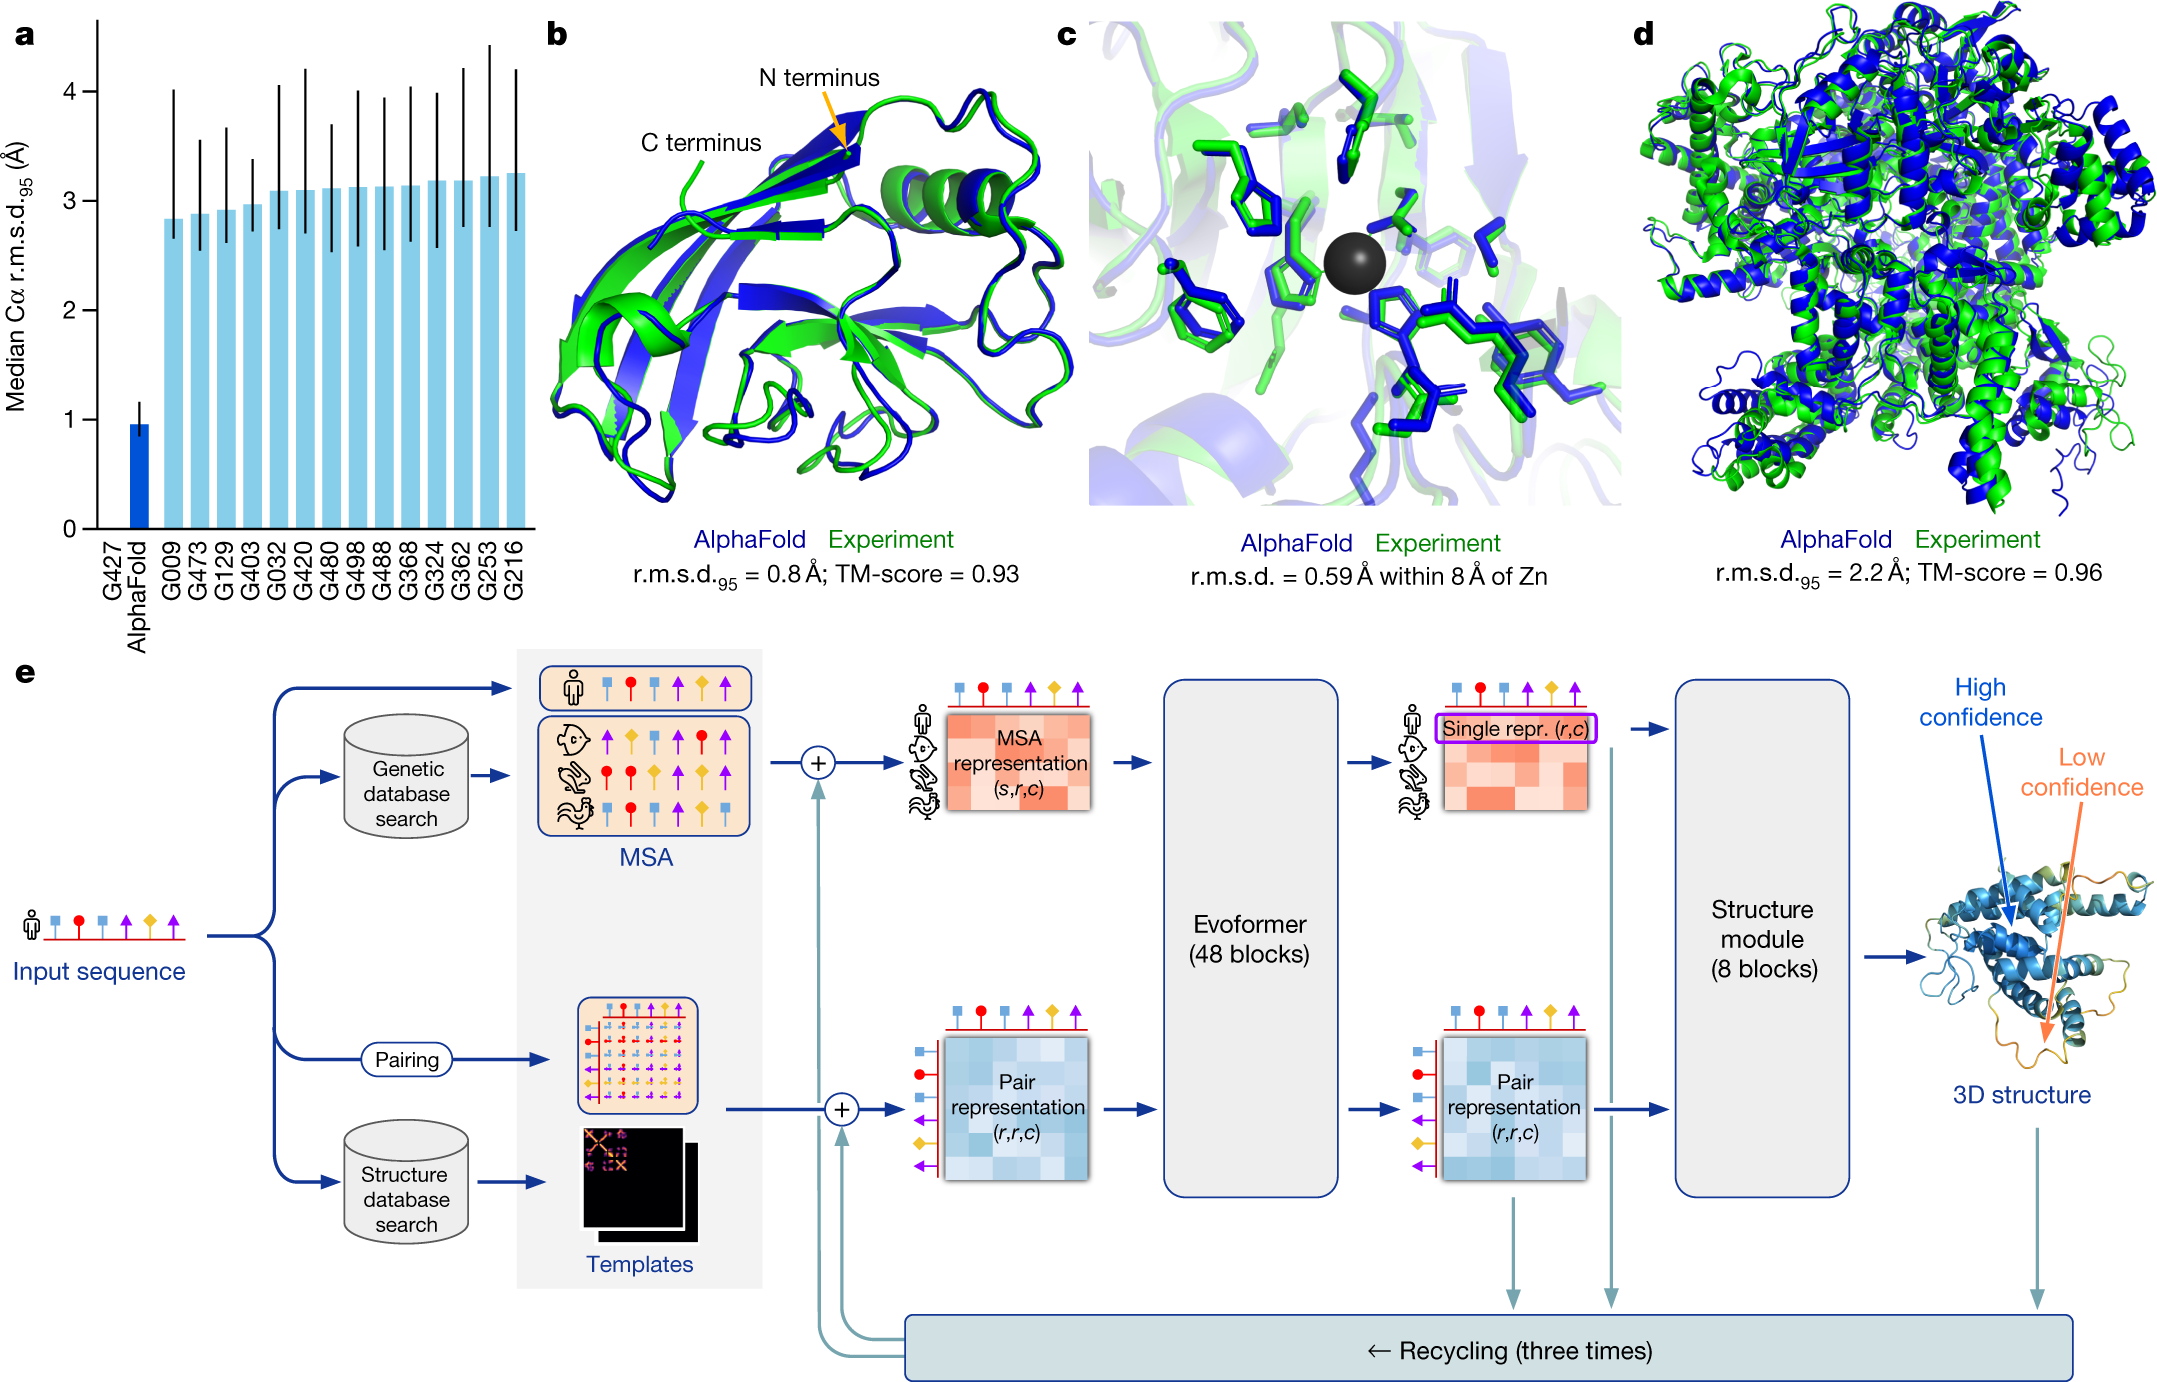
\includegraphics[width=0.7\linewidth]{fig/alphafold.png}}
        \end{figure}
\end{frame}


\begin{frame}{Data-driven scientific computing: Three Categories}
	\begin{itemize}
		\item 1. \textbf{100\% data-driven}: Physics-informed neural networks (PINN), Fourier neural operator, DeepONet.
		\item 2. \textbf{50 \% Numerical + 50 \% data-driven}: Machine learning turbulence modeling, DeepPotential, Quasipotential. 
		\item 3. \textbf{Discovering physics law from data}: Symbolic regression for conservation law, Principle component analysis for phase transition, cluster algorithm for space-time classification.
	\end{itemize}
\end{frame}


\begin{frame}{Data-driven for Reynolds stresses modeling}
	$\la \mfU \ra =$ time average of $\mfU$, $\mfu = \mfU - \la \mfU \ra$, Reynolds-averaged Navier-Stokes (RANS) equation reads
	\bequ
		\begin{aligned}
	\p_t \la \mfU \ra + (\la \mfU \ra \cdot \nabla)\la \mfU \ra + \frac{\p \la \mfu u_j \ra}{\p x_j} &= -\frac{1}{\rho}\nabla p + \nu \Delta \la \mfU \ra,		\\
	\nabla \cdot \la \mfU \ra &= 0.
	\end{aligned}
\eequ
Extra term: $\la \mfu u_j \ra$ (Reynolds stress). \textcolor{red}{\textbf{The equation is not closed}}!!
\par
Ling et al.\footnotemark proposed a data-driven surrogate model to estimate the Reynolds stresses.
\footnotetext{Ling, Julia, Andrew Kurzawski, and Jeremy Templeton. "Reynolds averaged turbulence modelling using deep neural networks with embedded invariance." Journal of Fluid Mechanics 807 (2016): 155-166.
}
\end{frame}


\begin{frame}{Improve the prediction of flow separation}
	\begin{figure}[H]
          \centering
          \centerline{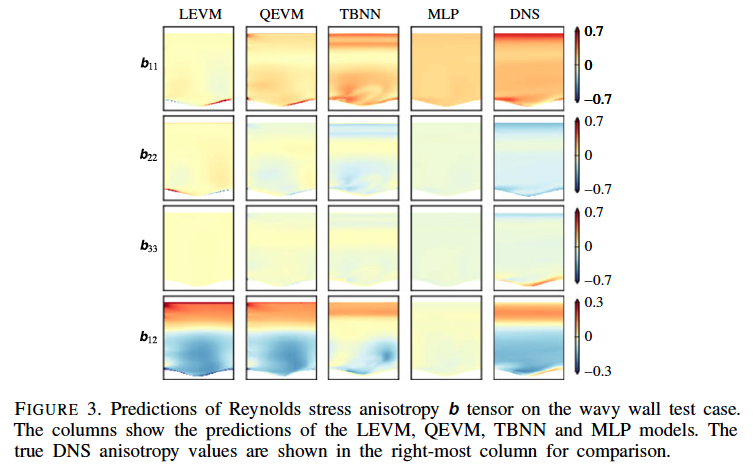
\includegraphics[width=\linewidth]{fig/tbnn.png}}
        \end{figure}
\end{frame}


\begin{frame}{Data-driven scientific computing: Our Focus}
	\begin{itemize}
		\item 1. \textbf{100\% data-driven}: Physics-informed neural networks (PINN), Fourier neural operator, DeepONet.
		\item 2. \textcolor{red}{\textbf{50 \% Numerical + 50 \% data-driven}: Machine learning turbulence modeling, DeepPotential, Quasipotential.} 
		\item 3. \textbf{Discovering physics law from data}: Symbolic regression for conservation law, Principle component analysis for phase transition.
	\end{itemize}
\end{frame}


\begin{frame}{Framework for the second approach}
	Simulating the dynamics:
	\bequn
		\begin{aligned}
			\p_t \mfx & = \mcL(\mfx, \mfu, t), \quad \mfx \in \mcX, \mfu \in \mcU, \mcL: \mcX \times \mcU \times \mbR_+ \rightarrow T\mcX,			\\
			\mfu & = \phi(\mfx, t), \quad \phi: \mcX \times \mbR_+ \rightarrow \mfu.
		\end{aligned}
	\eequn
	\begin{itemize}
		\item 1. $\mcL$ is known, possibly non-linear.
		\item 2. $\phi$ is un-known.
		\item 3. A set of data pairs $\lbb (\mfx_1, \mfu_1, t_1), (\mfx_2, \mfu_2, t_2), \cdots, (\mfx_N, \mfu_N, t_N )\rbb. $
		\item 4. Benchmark algorithm solves the ordinary least square:
		\bequn
			\arg\min_{\theta} \mbE \norml \mfu - \phi_{\theta}(\mfx, t) \normr^2.
		\eequn
	\end{itemize}

\end{frame}


\begin{frame}{Inner-outer loop: Linear outer loop}
In many scientific computing examples, further simplification:
\begin{align*}\label{linear-sys}
	\mfx_{k+1} & = A\mfx_{k} + B\mfu_k,\quad \mfx_k \in \mbR^n, \mfu_k \in \mbR^m,		\nonumber \\
	\mfu_k & = f(\mfx_k).
\end{align*}
\par
The outer loop is known to us and usually has some good numerical properties, i.e. linear, stable, etc, while the inner loop can be complicated.
\end{frame}


\begin{frame}{Inner-outer loop: examples}
\begin{Ex}[RANS]
\bequn
	\begin{aligned}
&\left\{\begin{aligned}
	\p_t \la \mfU \ra + (\la \mfU \ra \cdot \nabla)\la \mfU \ra + \nabla \cdot \tau &= -\frac{1}{\rho}\nabla p + \nu \Delta \la \mfU \ra,		\\
	\nabla \cdot \la \mfU \ra &= 0.
\end{aligned}\right.		\\
&\tau = R(\la \mfU \ra).
\end{aligned}
\eequn
\end{Ex}
\begin{Ex}[Quasi-potential]
\begin{align}\label{qp}
	\mfx_{k+1} & = \mfx_{k} - \Delta t\mfu_k,		\nonumber \\
	\mfu_k & = \nabla V_{\theta}(\mfx_k) + g_{\theta}(\mfx_k).
\end{align}
\end{Ex}

\end{frame}


\begin{frame}{Dilemma of data-driven scientific computing}
	In the data-driven scientific computing, \textcolor{red}{\textbf{dynamics structure}} can cause \textcolor{red}{\textbf{distribution mismatch}} between the training and testing data.
	\begin{figure}[H]
          \centering
          \centerline{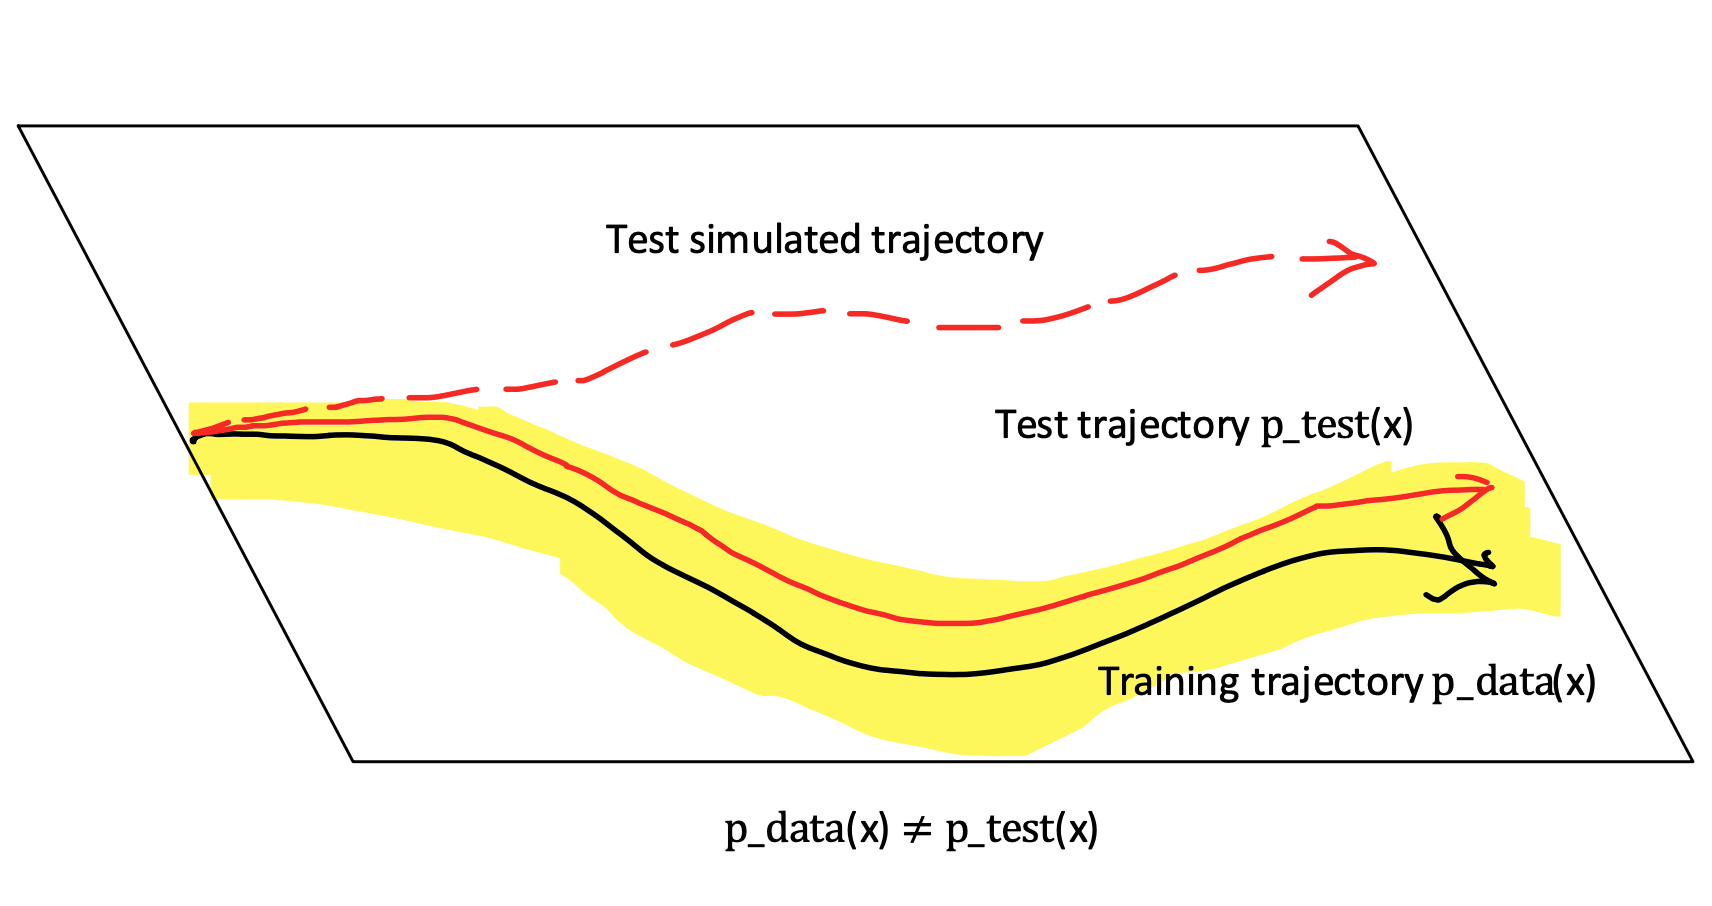
\includegraphics[width=\linewidth]{fig/dilemma.png}}
        \end{figure}
\end{frame}


\begin{frame}{Algorithm to mitigate the distribution mismatch}
	Modified the training dataset to mitigate the distribution shift.
	\begin{figure}[H]
          \centering
          \centerline{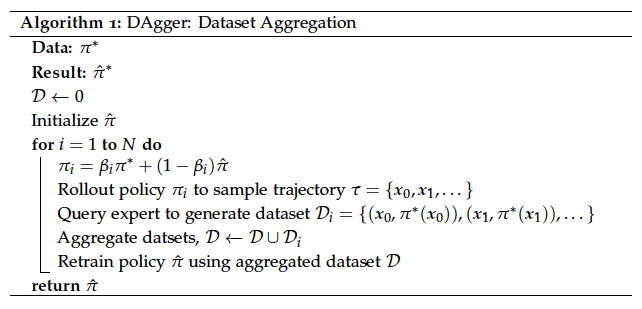
\includegraphics[width=\linewidth]{fig/DAgger.png}}
        \end{figure}
\end{frame}


\begin{frame}{Algorithm to mitigate the distribution mismatch}
	\begin{figure}[H]
          \centering
          \centerline{\includegraphics[width=\linewidth]{fig/DAggerpic.png}}
        \end{figure}
\end{frame}


\begin{frame}{An intuition}	
	\bequn
		\begin{aligned}
			\p_t \mfx & = \mcL(\mfx, \mfu, t), \quad \mfx \in \mcX, \mfu \in \mcU, \mcL: \mcX \times \mcU \times \mbR_+ \rightarrow T\mcX,			\\
			\mfu & = \phi(\mfx, t), \quad \phi: \mcX \times \mbR_+\rightarrow \mfu.
		\end{aligned}
	\eequn
	Ordinary least square $\norml \mfu - \phi(\mfx, t) \normr^2$ cannot distinguish the following case. Add regularization for this as $R(\wht \mfx)$ where $\wht \mfx$ is next state variable given current state $\mfx$ and control $\mfu$, i.e. $\wht \mfx = \mfx + \mcL(\mfx, \mfu, t)dt$.
	\begin{figure}[H]
          \centering
          \centerline{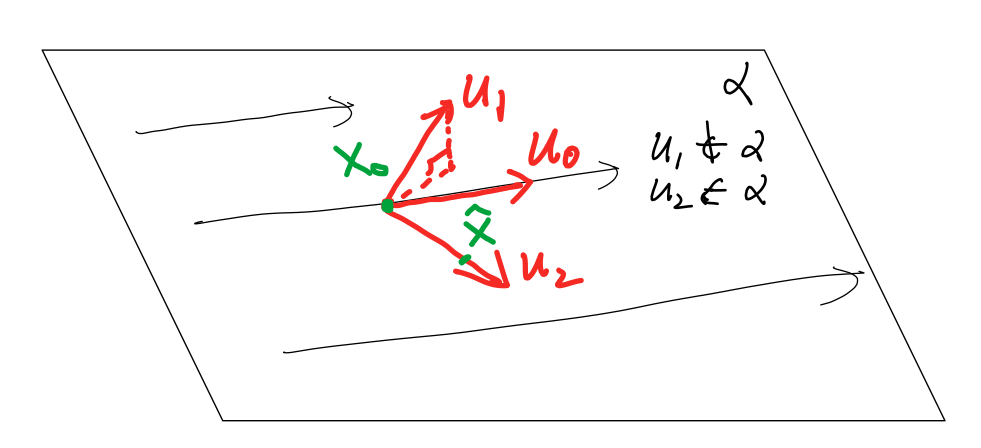
\includegraphics[width=0.9\linewidth]{fig/mfd.png}}
        \end{figure}
\end{frame}


\begin{frame}{Theoretic analysis: linear case}
	\begin{Thm}
		Consider the following least square problem $\mfY = \beta \mfX, \mfY \in \mbR^{m\times n}, \beta \in \mbR^{m\times m}, \mfX \in \mbR^{m\times n}$. Furthermore, we suppose that the data $X_i$ lies in a hyperplane of codimension $r$ given by:
		\bequn
			c_i^T X_j = d_i, \forall i, j.
		\eequn
		Then the regularized estimator proposed is given by
		\bequn
			\wht \beta = (\mfI + \lambda \mfC \mfC^T)^{-1} \mfY\mfX^T (\mfX\mfX)^{\dagger}.
		\eequn
	\end{Thm}
\end{frame}


\begin{frame}{Theoretic analysis}
	\begin{Thm}[Informal]
		Assume that the simulated trajectories will not be far away from the data manifold, i.e. $d(\wht X_i, \mcM) = o(1)$. The data driven solver will be convergent, i.e. $d(\wht X_T, X_T) \rightarrow 0$ as samples tends to infinity.
	\end{Thm}
\end{frame}


\begin{frame}{Algorithms and numerical experiments}
	Linear control:
	\begin{equation}
    \begin{aligned}
        \dot{x}_t & = v_t, \\
        \dot{v}_t & = -\alpha(t) v_t + u_t,	\\
        	x_0 & = 1, v_0 = 0,		\\
	x_1 & = 0,			\\
	\alpha(t) & = \sin 10 t.
    \end{aligned}
\end{equation}
And we use a \textbf{neural network} with $2$ hidden layer to parameterize the mapping from $(x_k, v_k, t_k)$ to $u_k$. Hence the neurons in each layer is given by $3, n, n, 1$ where $n$ can be varied in the experiments.
\end{frame}


\begin{frame}{Algorithms and numerical experiments}
	Inner-Outer loop structure of this linear control:
	\begin{equation}
		\begin{aligned}
			\begin{pmatrix} x_{k+1} \\ v_{k+1}
			\end{pmatrix} & \ = \begin{pmatrix} 1 & dt \\ 0 & 1-\alpha_k dt
			\end{pmatrix}\begin{pmatrix} x_{k} \\ v_{k}
			\end{pmatrix} + \begin{pmatrix} 0 \\ 1
			\end{pmatrix}u_k,		\\
			u_k & \ = \phi_{NN}(x_k, v_k, t_k).
		\end{aligned}
	\end{equation}
	And ordinary least square (behavior cloning) simply solve the model by minimizing the following function:
	$$l(\phi_{NN}(x_k, v_k, t_k), u_k) = \norml \phi_{NN}(x_k, v_k, t_k) - u_k \normr_2^2.$$
\end{frame}


\begin{frame}{Bench mark: Ordinary least square}
	Averaged error is given by $0.192341$.
	\begin{figure}[H]
          \centering
          \centerline{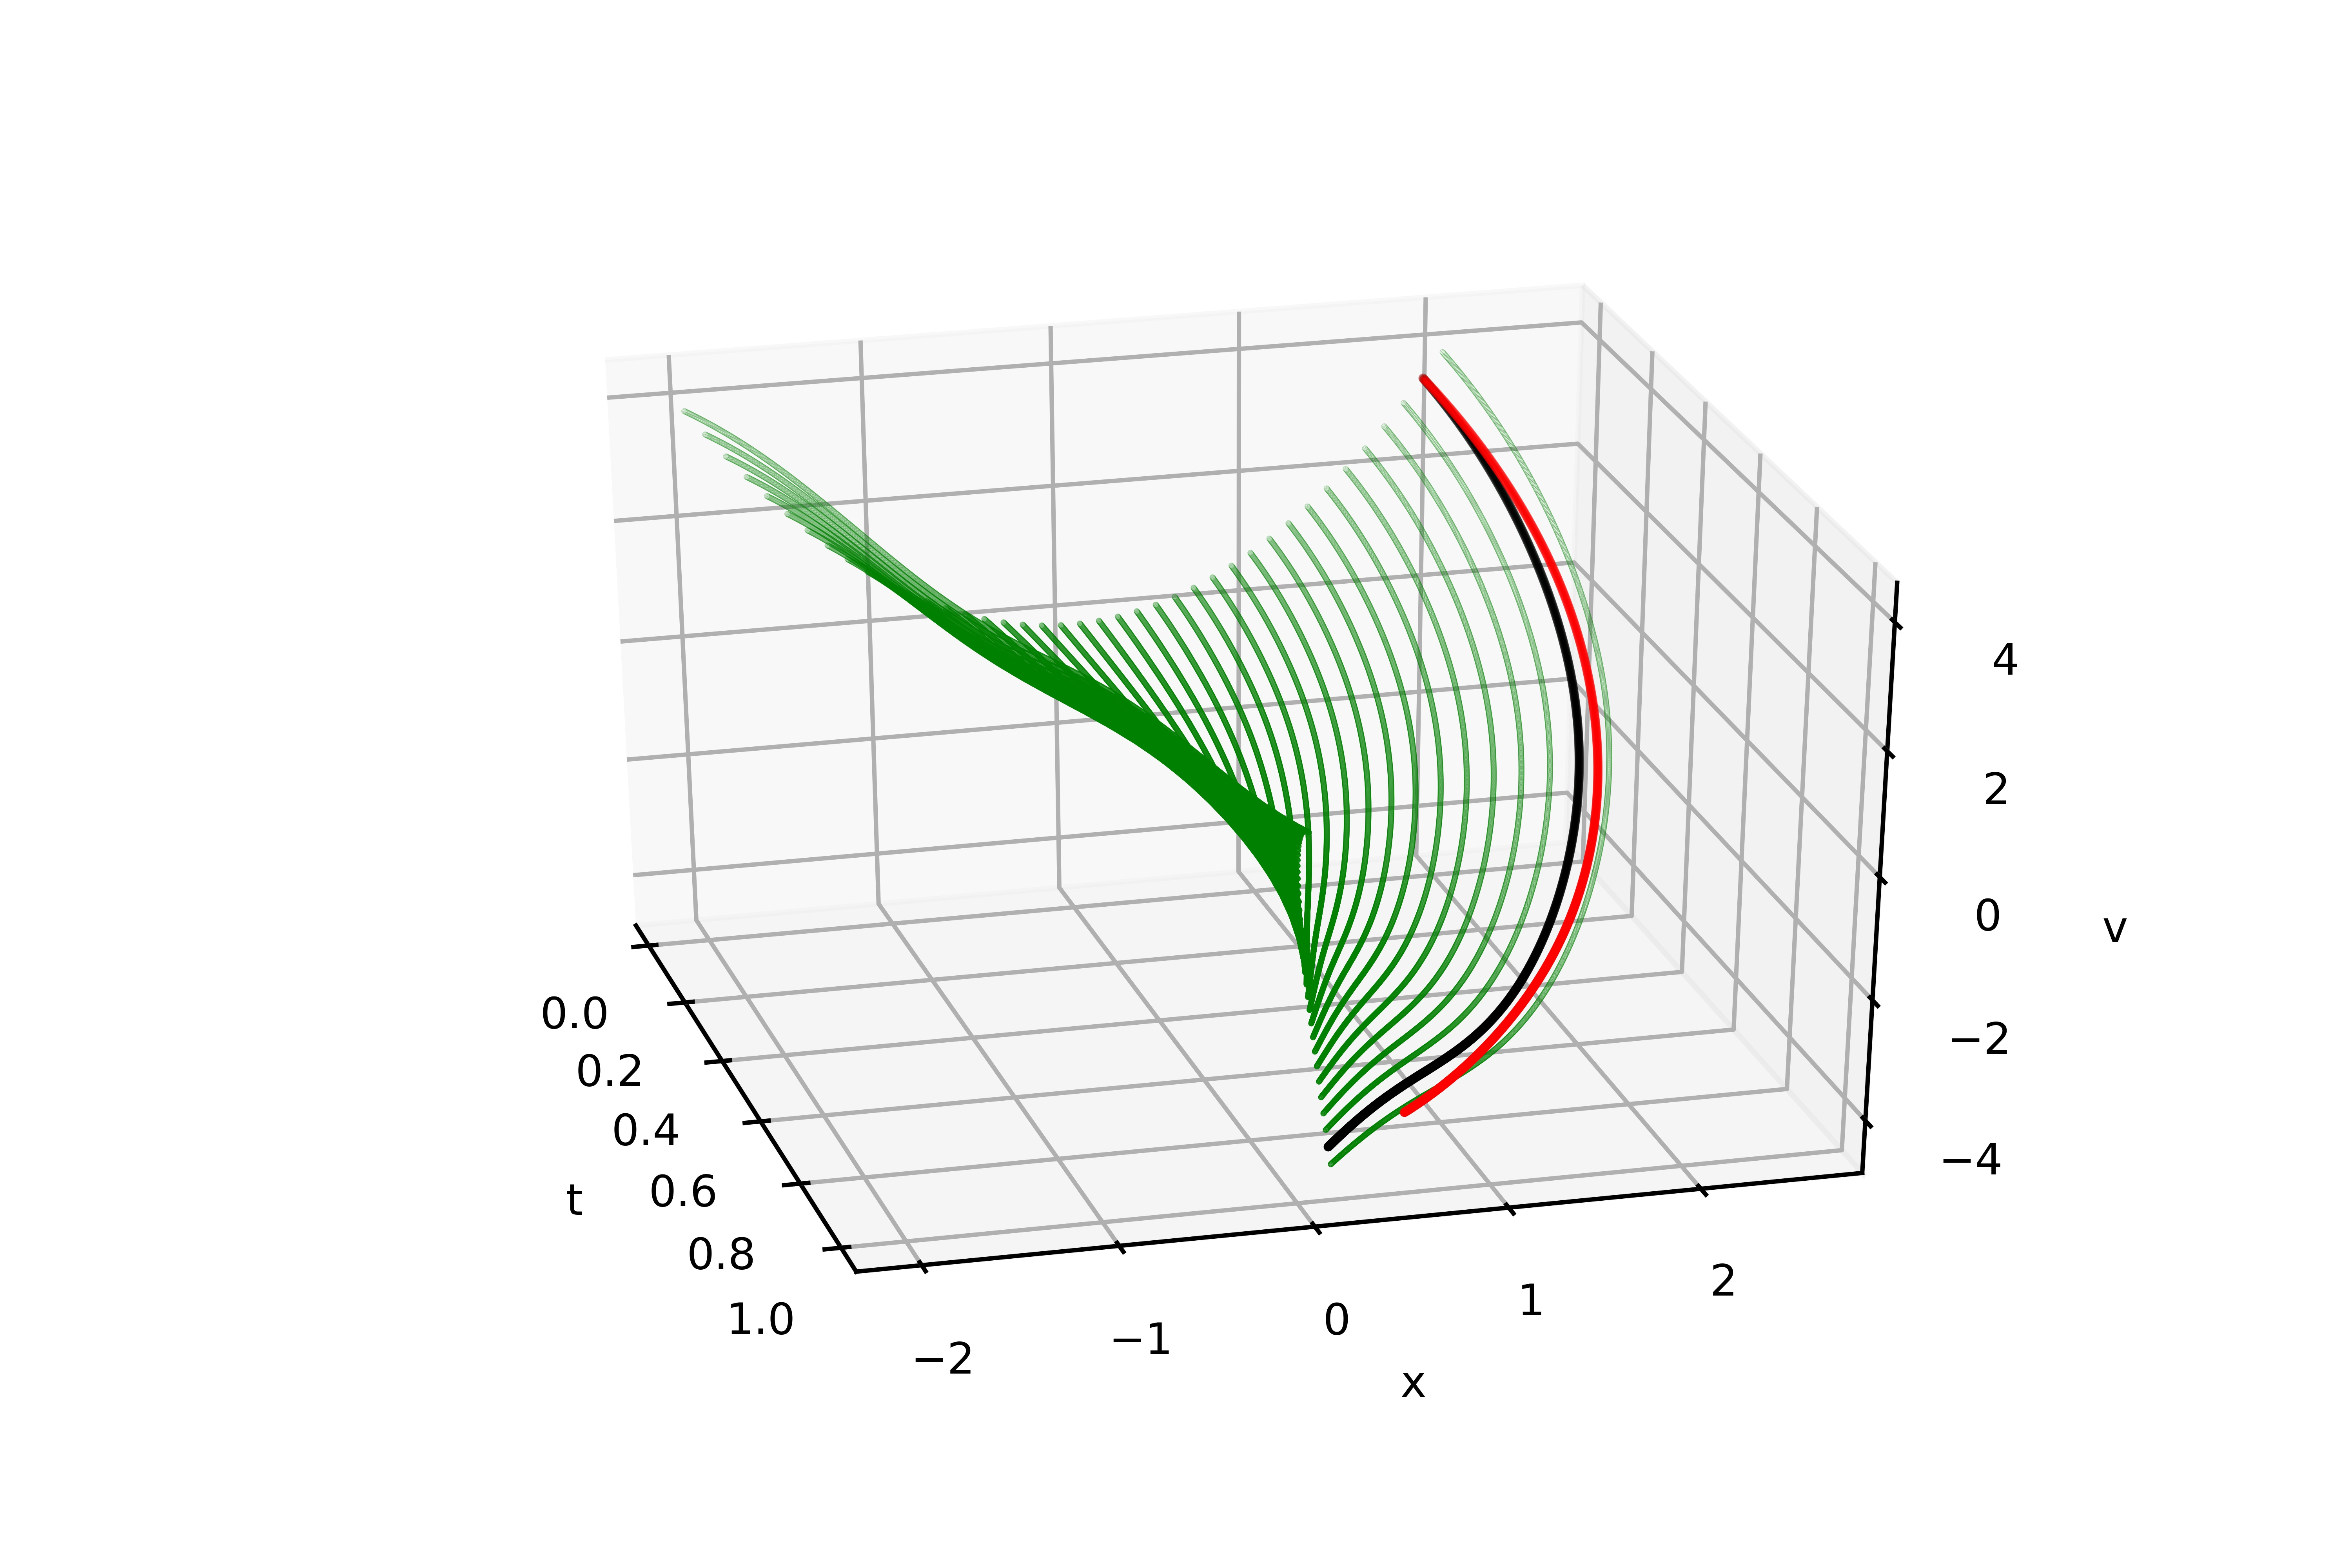
\includegraphics[width=0.7\linewidth]{fig/control1-1.jpg}}
          \caption{Sampled training trajectory of an estimator with underlying net of 		10 hidden neurons.}
	\end{figure}
\end{frame}


\begin{frame}{Manifold regularization}
	Several choices of empirical manifold:
	\begin{itemize}
		\item Formed by the sample trajectories in the training data, i.e.
	\bequn
		\mcM_t := \lbb (x(t), v(t), t)  \quad t \in [0, 1]  \rbb,
	\eequn
		\item The other empirical manifold related to the data-driven surrogate model
		 and can be defined as following set:
\bequn
	\wht \mcM_t := \lbb (x, v, t) \Big| \norml \phi_{NN}(x_k, v_k, t_k) - u_k \normr_2 < \epsilon \rbb.
\eequn
	
\end{itemize}
\end{frame}


\begin{frame}{$ \mcM_t $}
\bequn
		\min_{\theta} \mbE \norml \mfu - \phi_{\theta}(\mfx, t) \normr^2 + \lambda
		 \norml D(E(\wht \mfx)) - \wht \mfx \normr^2
	\eequn
	Averaged error is given by $0.173001$.
	\begin{figure}[H]
          \centering
          \centerline{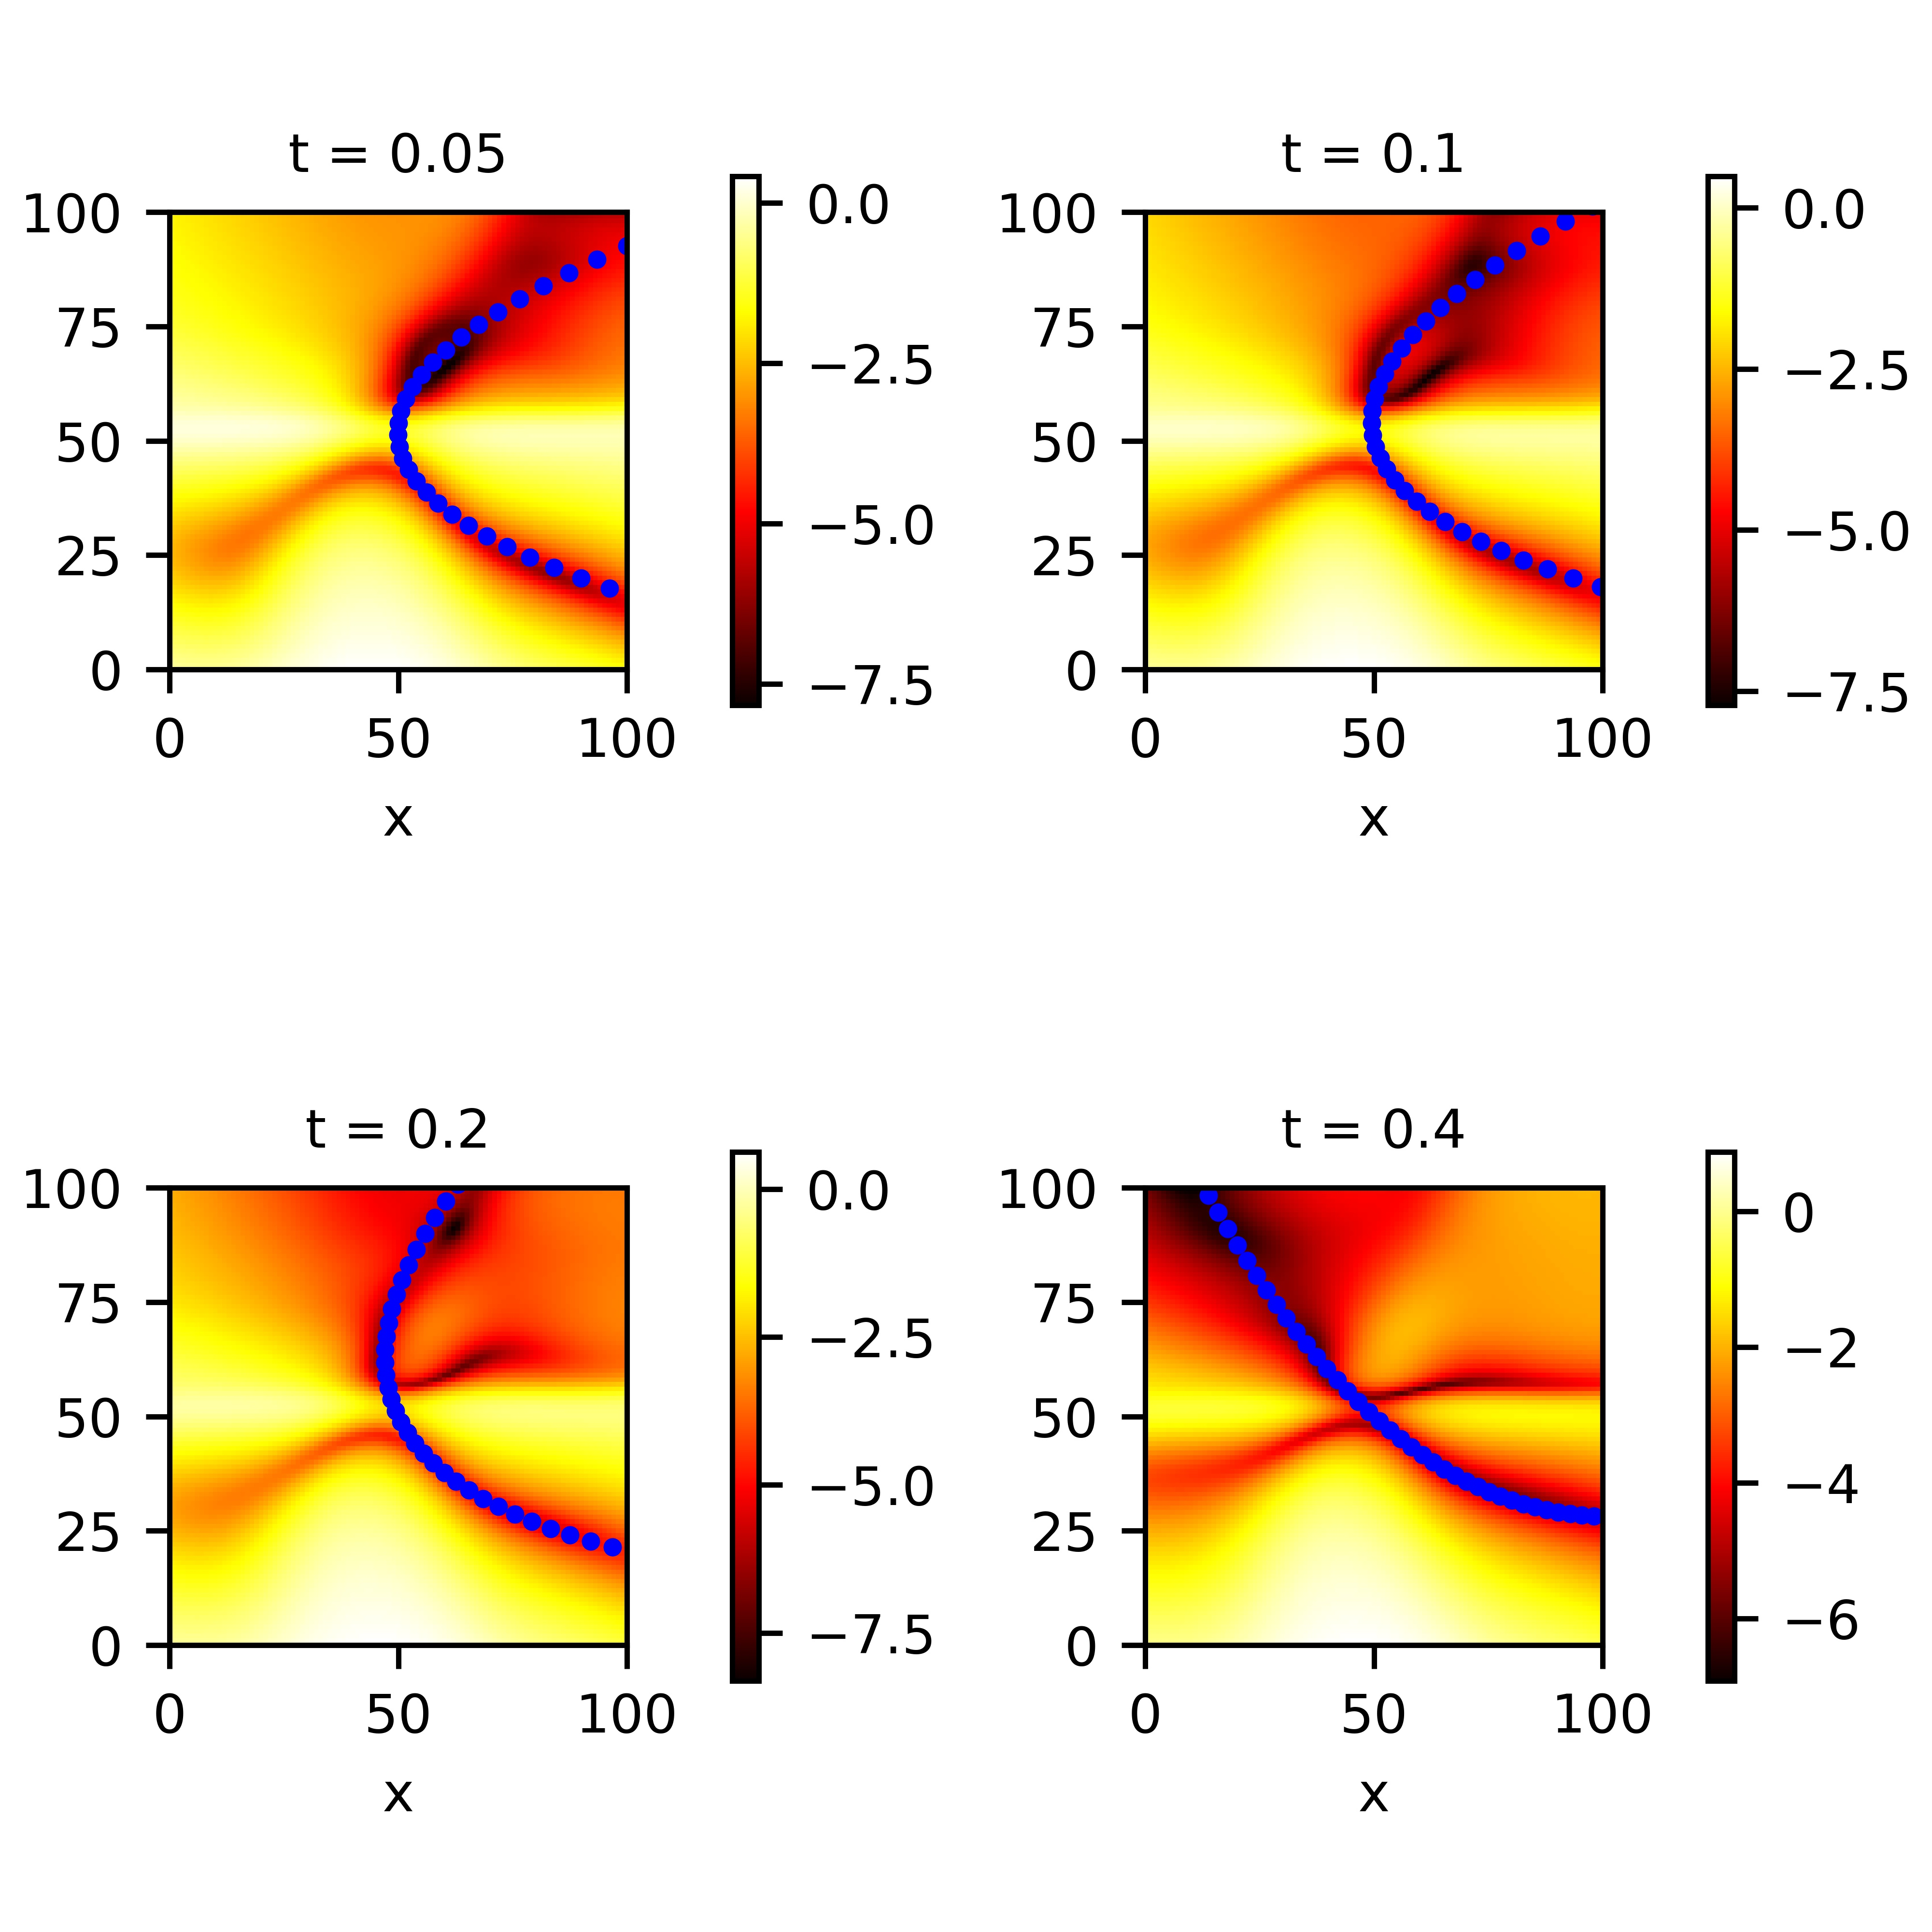
\includegraphics[width=0.65\linewidth]{fig/control6.jpg}}
          \label{l2-mfd}
\end{figure}
\end{frame}


\begin{frame}{$\wht \mcM_t $}
	\bequn
		\min_{\theta} \mbE \norml \mfu - \phi_{\theta}(\mfx, t) \normr^2 + \lambda
		 \norml \wht \mfu - \phi_{\theta}(\wht \mfx, t) \normr^2
	\eequn
	Averaged error is given by $0.160128$.
	\begin{figure}[H]
          \centering
          \centerline{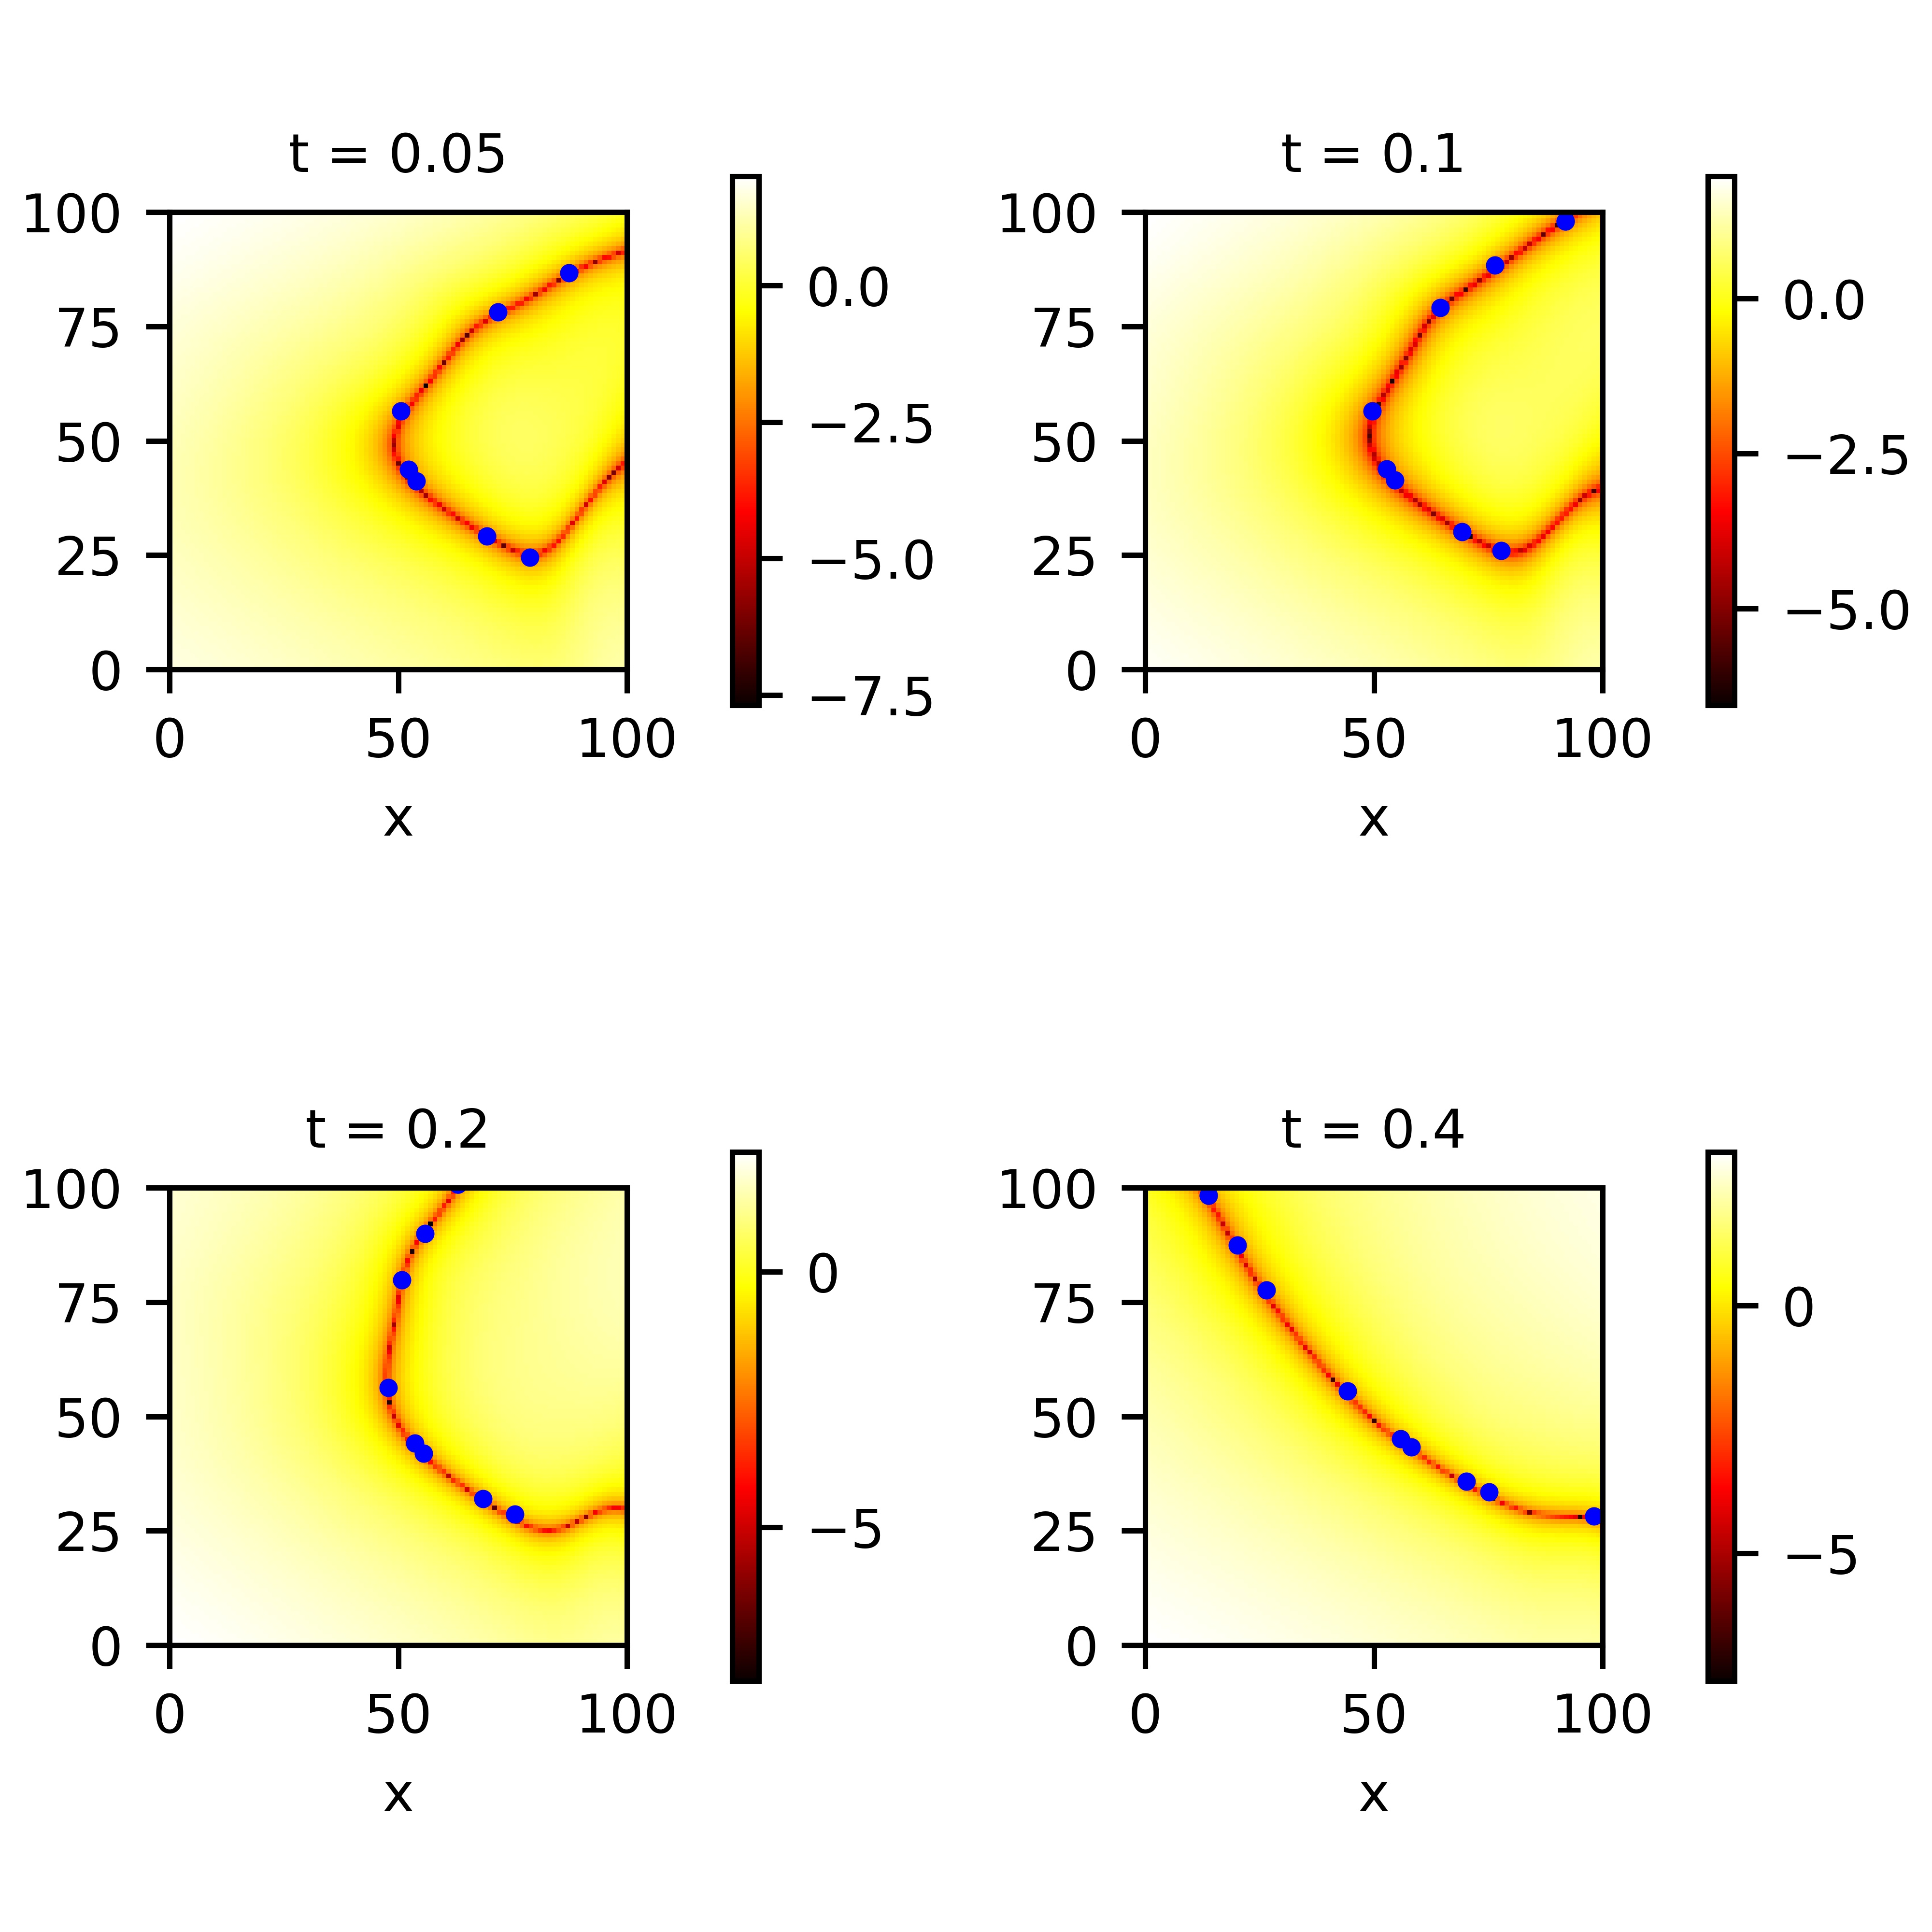
\includegraphics[width=0.65\linewidth]{fig/control4.jpg}}
          \label{l2-mfd}
	\end{figure}
\end{frame}


\begin{frame}{Reaction Diffusion equation}
	Consider following FitzHugh-Nagumo reaction diffusion (RD) equation:
	\begin{equation}\label{FN}
    \begin{aligned}
        	\frac{\p \mfu}{\p t} & = \gamma \Delta \mfu + \mfR(\mfu), \quad T \in [0, 1], 	\\
		\mfR(\mfu) & = \mfR(u, v) = \begin{pmatrix}
			u - u^3 - v - \alpha	\\
			\beta(u - v)
		\end{pmatrix},
    \end{aligned}
	\end{equation}
	This provides a simple inner-outer loop structure for the numerical solver.
	 The initial data is given by $\mfu_0$ is a random field and generated by i.i.d.
	  sampling from a normal distribution and $\alpha = 0.01, \beta=0.25$. We use
		 mesh size $128 \times 128$ for the whole problems. Computational domain is
		  given by $[0, 1]\times[0, 1]$.
\end{frame}


\begin{frame}{Fine-coarse grid}
	Another loop structure can be formulated as follows:
	\bequn
	\begin{aligned}
	I_n^{2n}: \mbR^{n \times n} \rightarrow \mbR^{2n \times 2n}			\\
	R_{2n}^{n}: \mbR^{2n \times 2n} \rightarrow \mbR^{n \times n}.
	\end{aligned}
\eequn
	\bequ
	\lbb\begin{aligned}
		\mfu_{2n}^{t+1} & = I_n^{2n} \circ f(R_{2n}^{n}(\mfu_{2n}^t)) + \wht \mfR(\mfu_{2n}^t),		\\
		\wht \mfR(\mfu) & = \phi_{NN}(u, v).
	\end{aligned}\right.
\eequ
	It is akin to the main idea of multigrid. Inner-loop now represents the role of
	 accounting for the residue of switching between two grid size.
\end{frame}


\begin{frame}{Network architecture}
	We choose U-net for 
	\begin{figure}[H]
          \centering
          \centerline{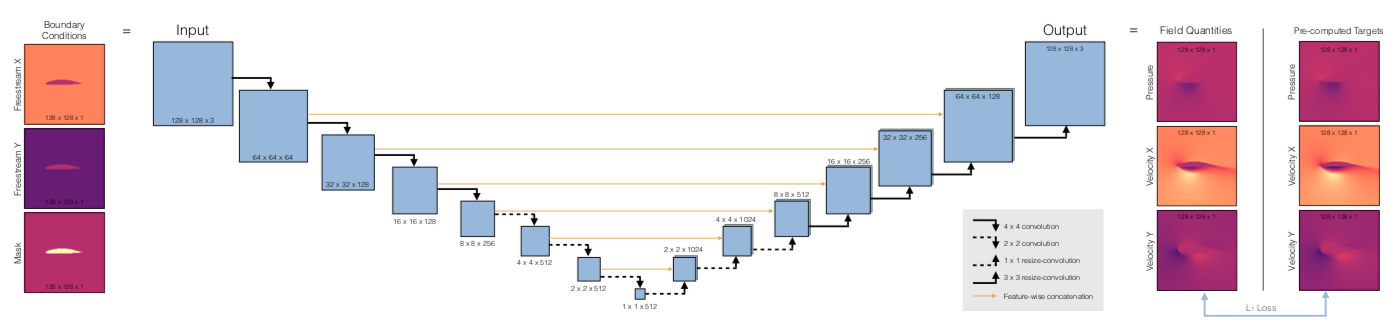
\includegraphics[width=1.1\linewidth]{fig/Unet.png}}
          \caption{U-net structure for flow prediction\footnotemark}
\end{figure}
\footnotetext{Thuerey, Nils, et al. "Deep learning methods for Reynolds-averaged
 Navier–Stokes simulations of airfoil flows." AIAA Journal 58.1 (2020): 25-36.}
\end{frame}


\begin{frame}{Simulation}
	On average in $200$ experiments, the regularized simulator improves by 40\%.
	\begin{figure}[H]
          \centering
          \centerline{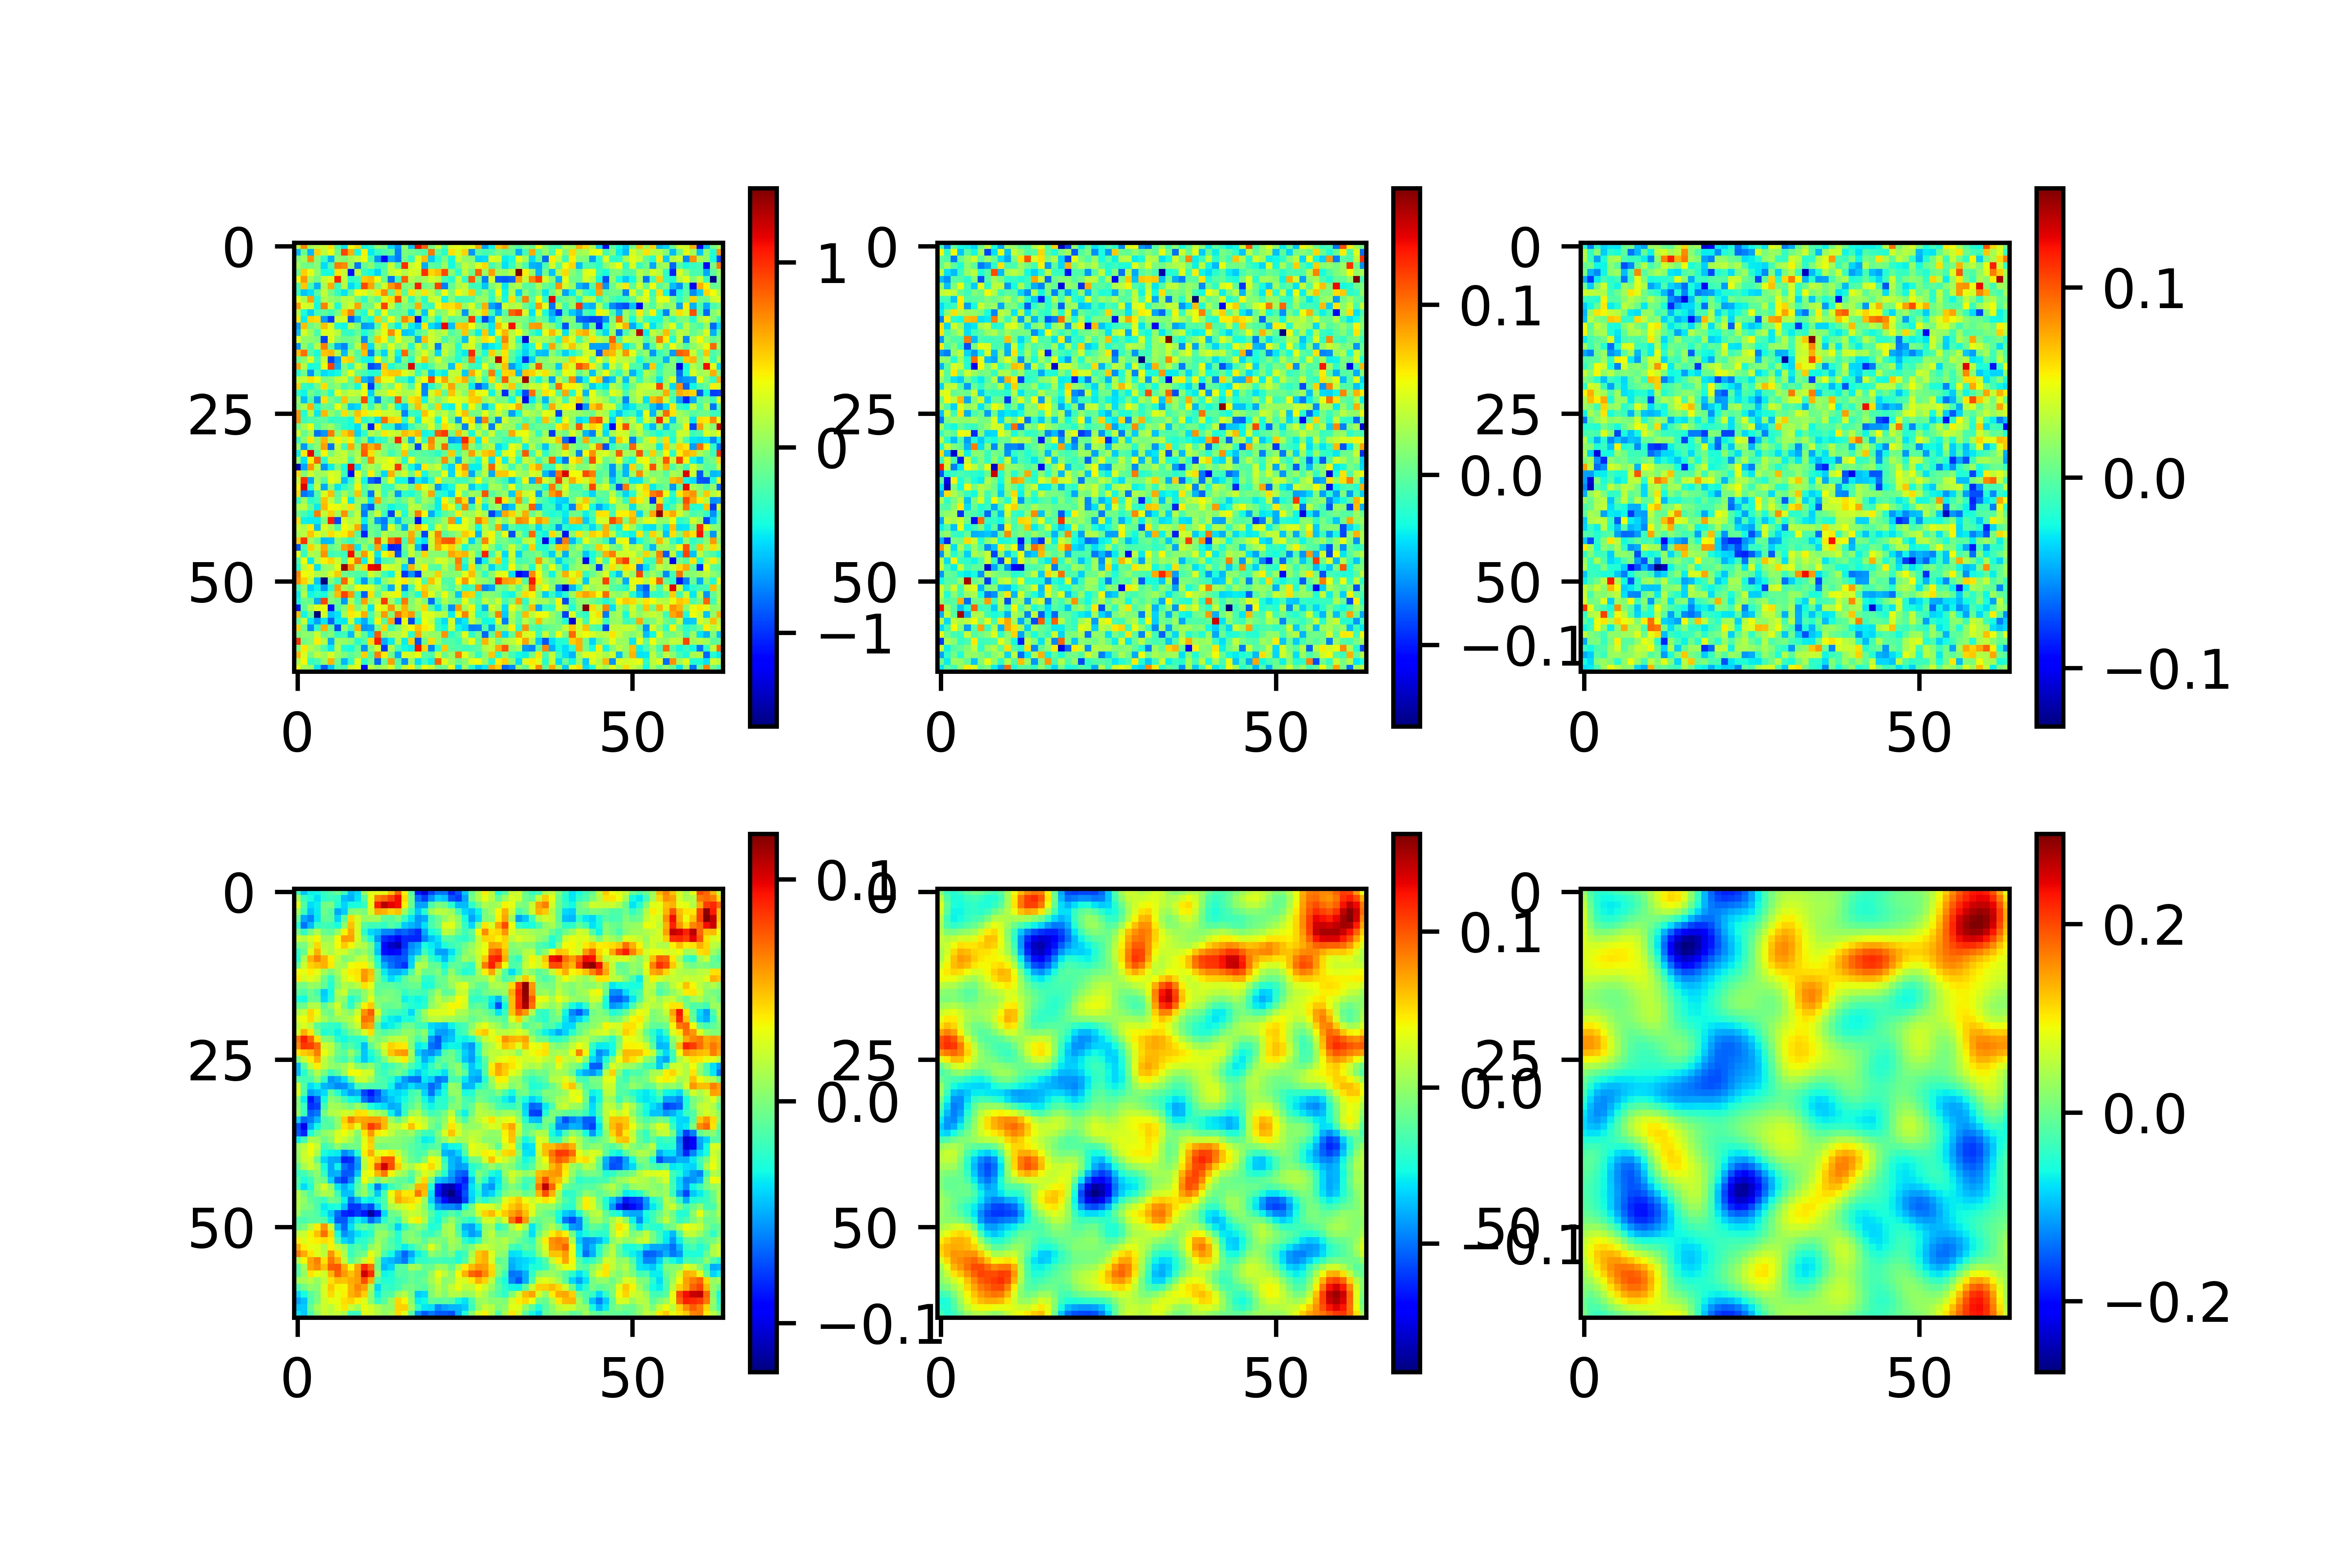
\includegraphics[width=0.4\linewidth]{fig/RD2-64-bm.jpg}}
          \centerline{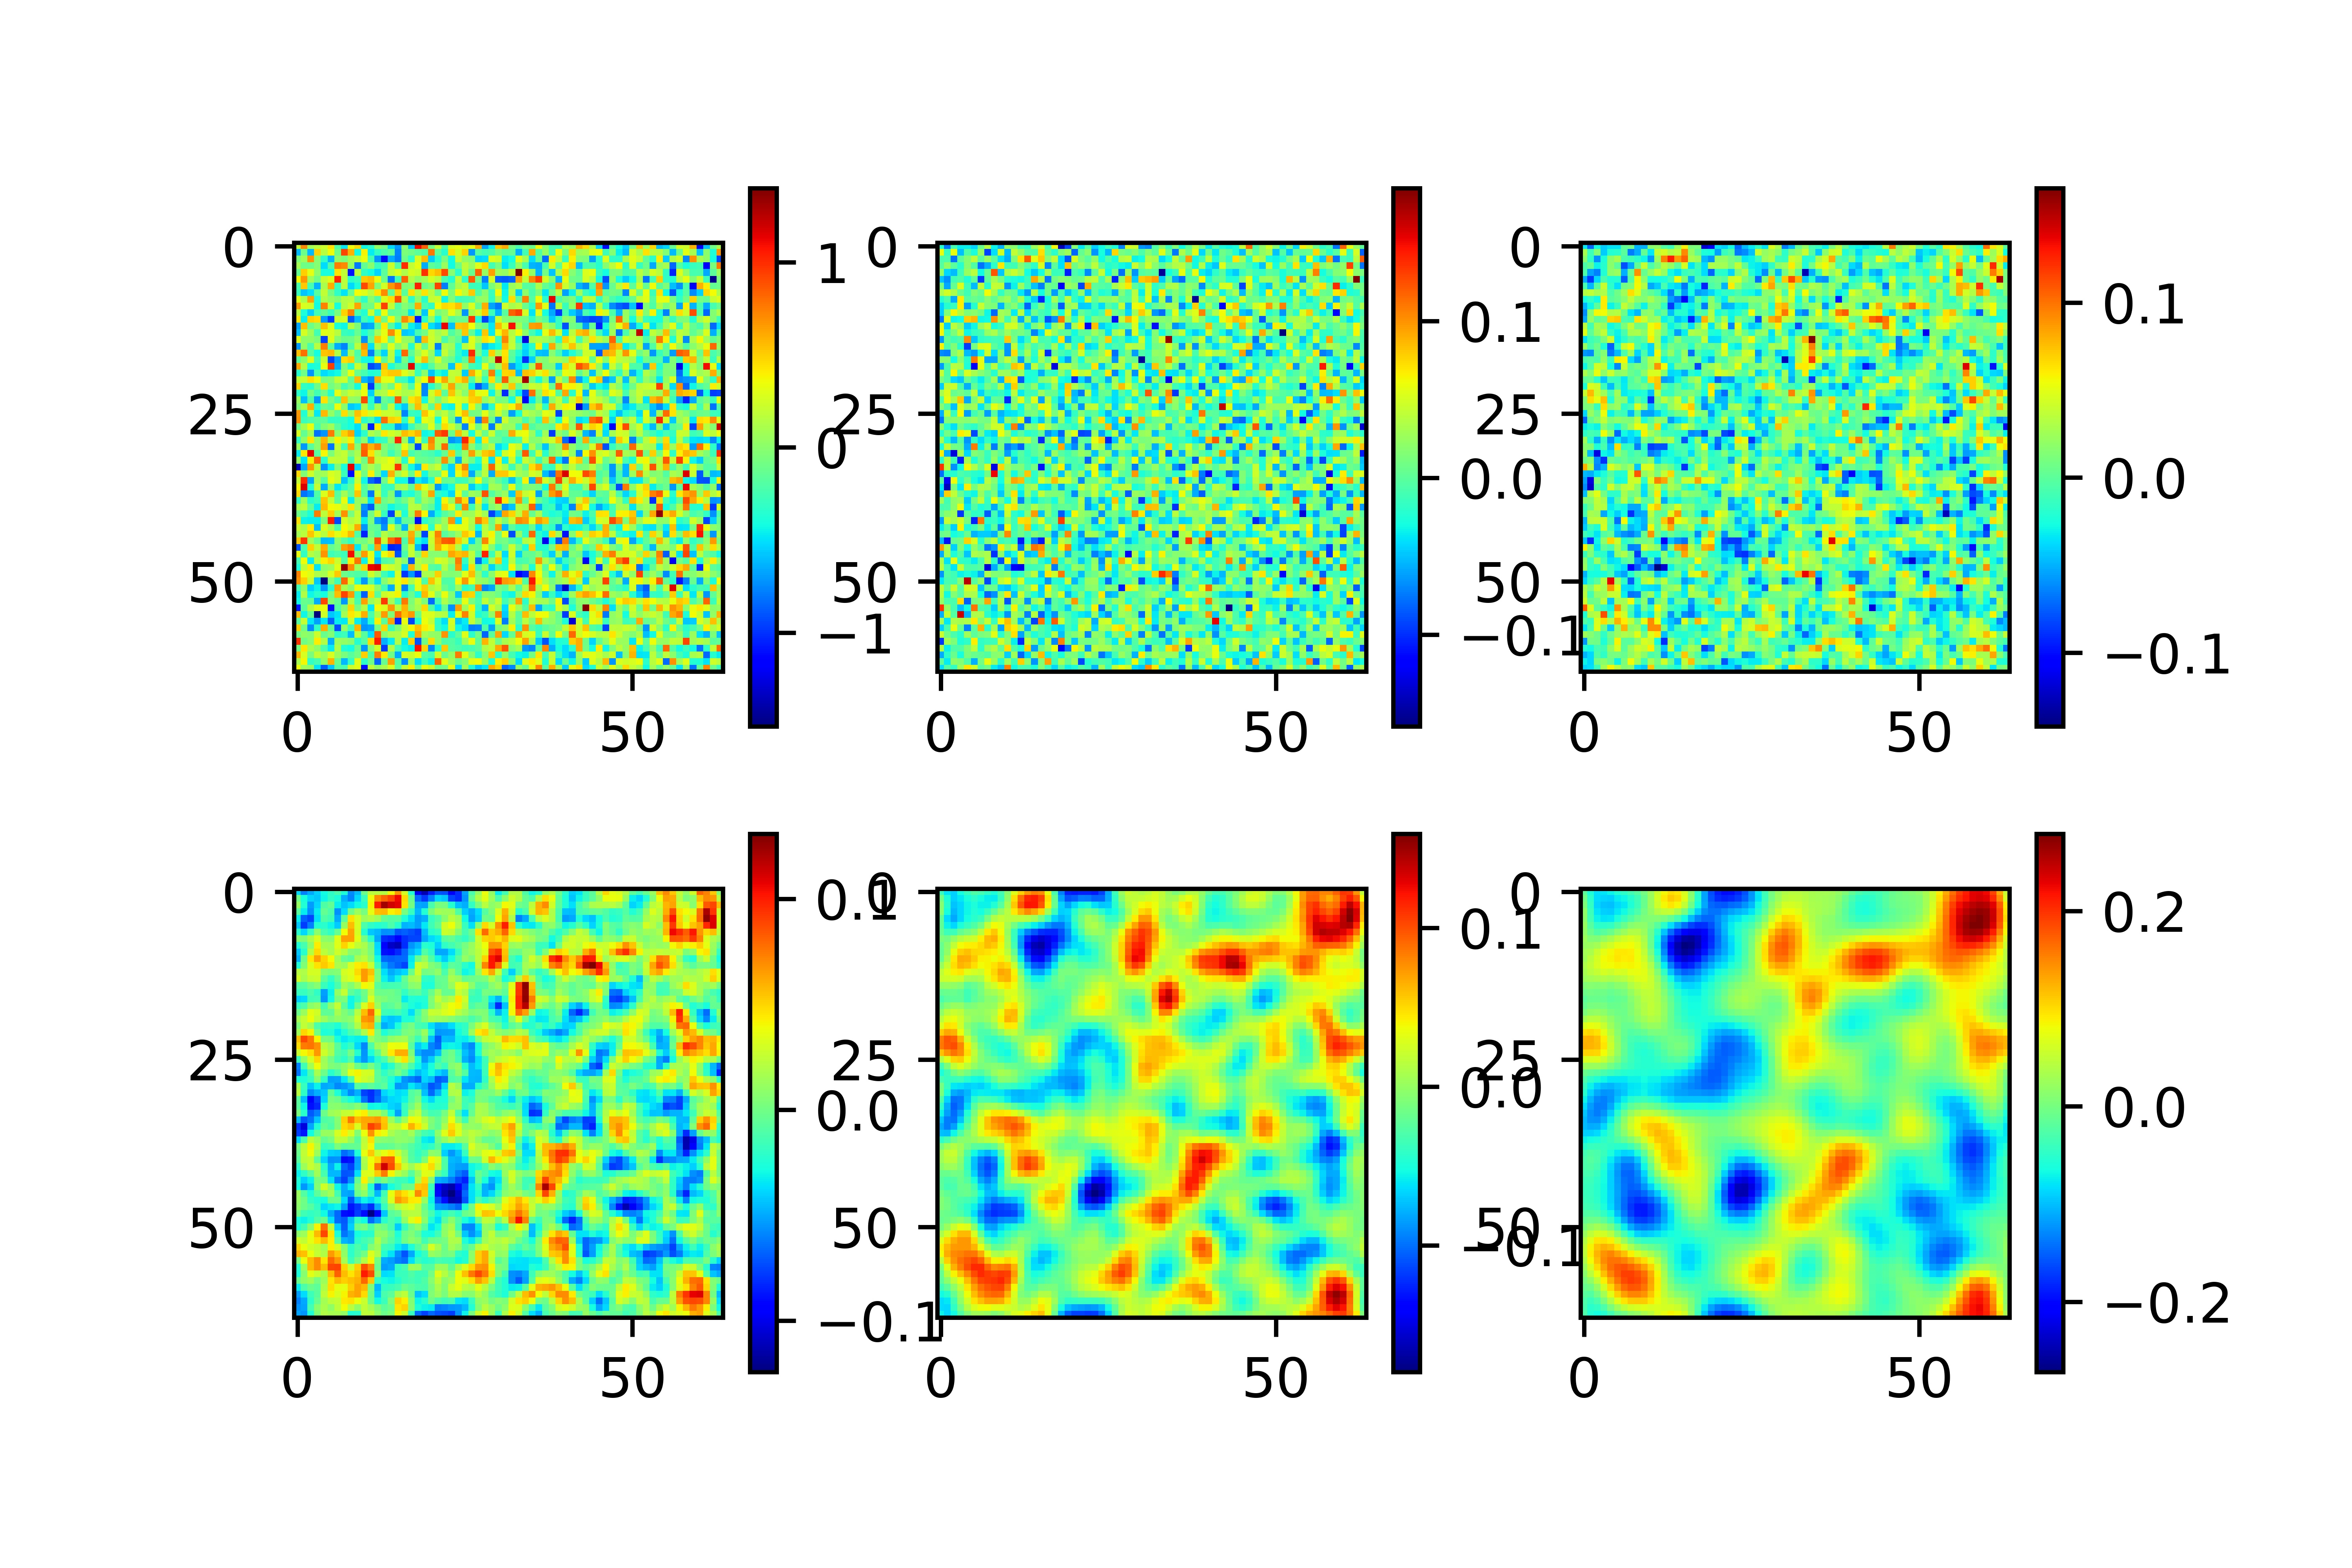
\includegraphics[width=0.4\linewidth]{fig/RD2-64-reg.jpg}}
          \caption{Upper: Benchmark with relative numerical error 12; Lower:
					 Regularized sampler with numerical error 8.}
\end{figure}
\end{frame}


\begin{frame}{Incompressible Navier-Stokes equation}
	Consider incompressible NS equation:
	\begin{equation}\label{FN}
    \begin{aligned}
        	\frac{\p \mfu}{\p t} + (\mfu \cdot \nabla)\mfu -  \nu \Delta \mfu & =
					\nabla p, \quad T \in [0, 1], 	\\
		\nabla \cdot \mfu & = 0,
    \end{aligned}
\end{equation}
	The computational domain is a rectangular $[0, 4]\times [0, 1]$. The boundary
	condition on upper and lower boundary is no-slip for velocity. The boundary condition
	for outlet is zero-gradient on pressure while we specify the inlet velocity.
\end{frame}


\begin{frame}{Typical flow configuration}
	\begin{figure}[H]
          \centering
          \centerline{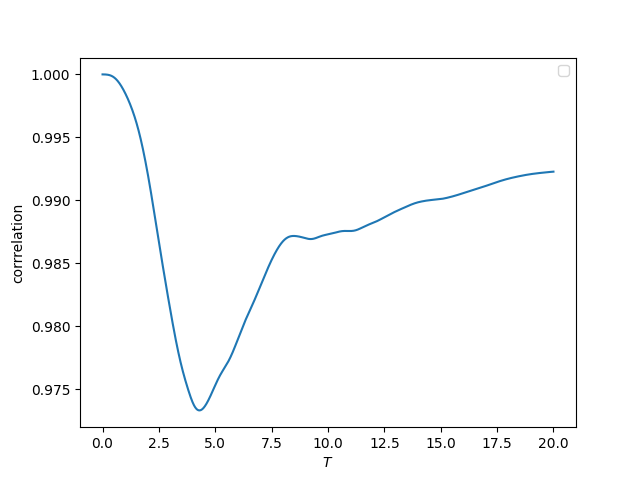
\includegraphics[width=0.6\linewidth]{fig/ns.png}}
          \caption{Simulation with time step 0.01 for time $20$, mesh size $128 \times 32$}
\end{figure}
\end{frame}


\begin{frame}{Prediction of the pressure}
	\begin{figure}[H]
          \centering
          \centerline{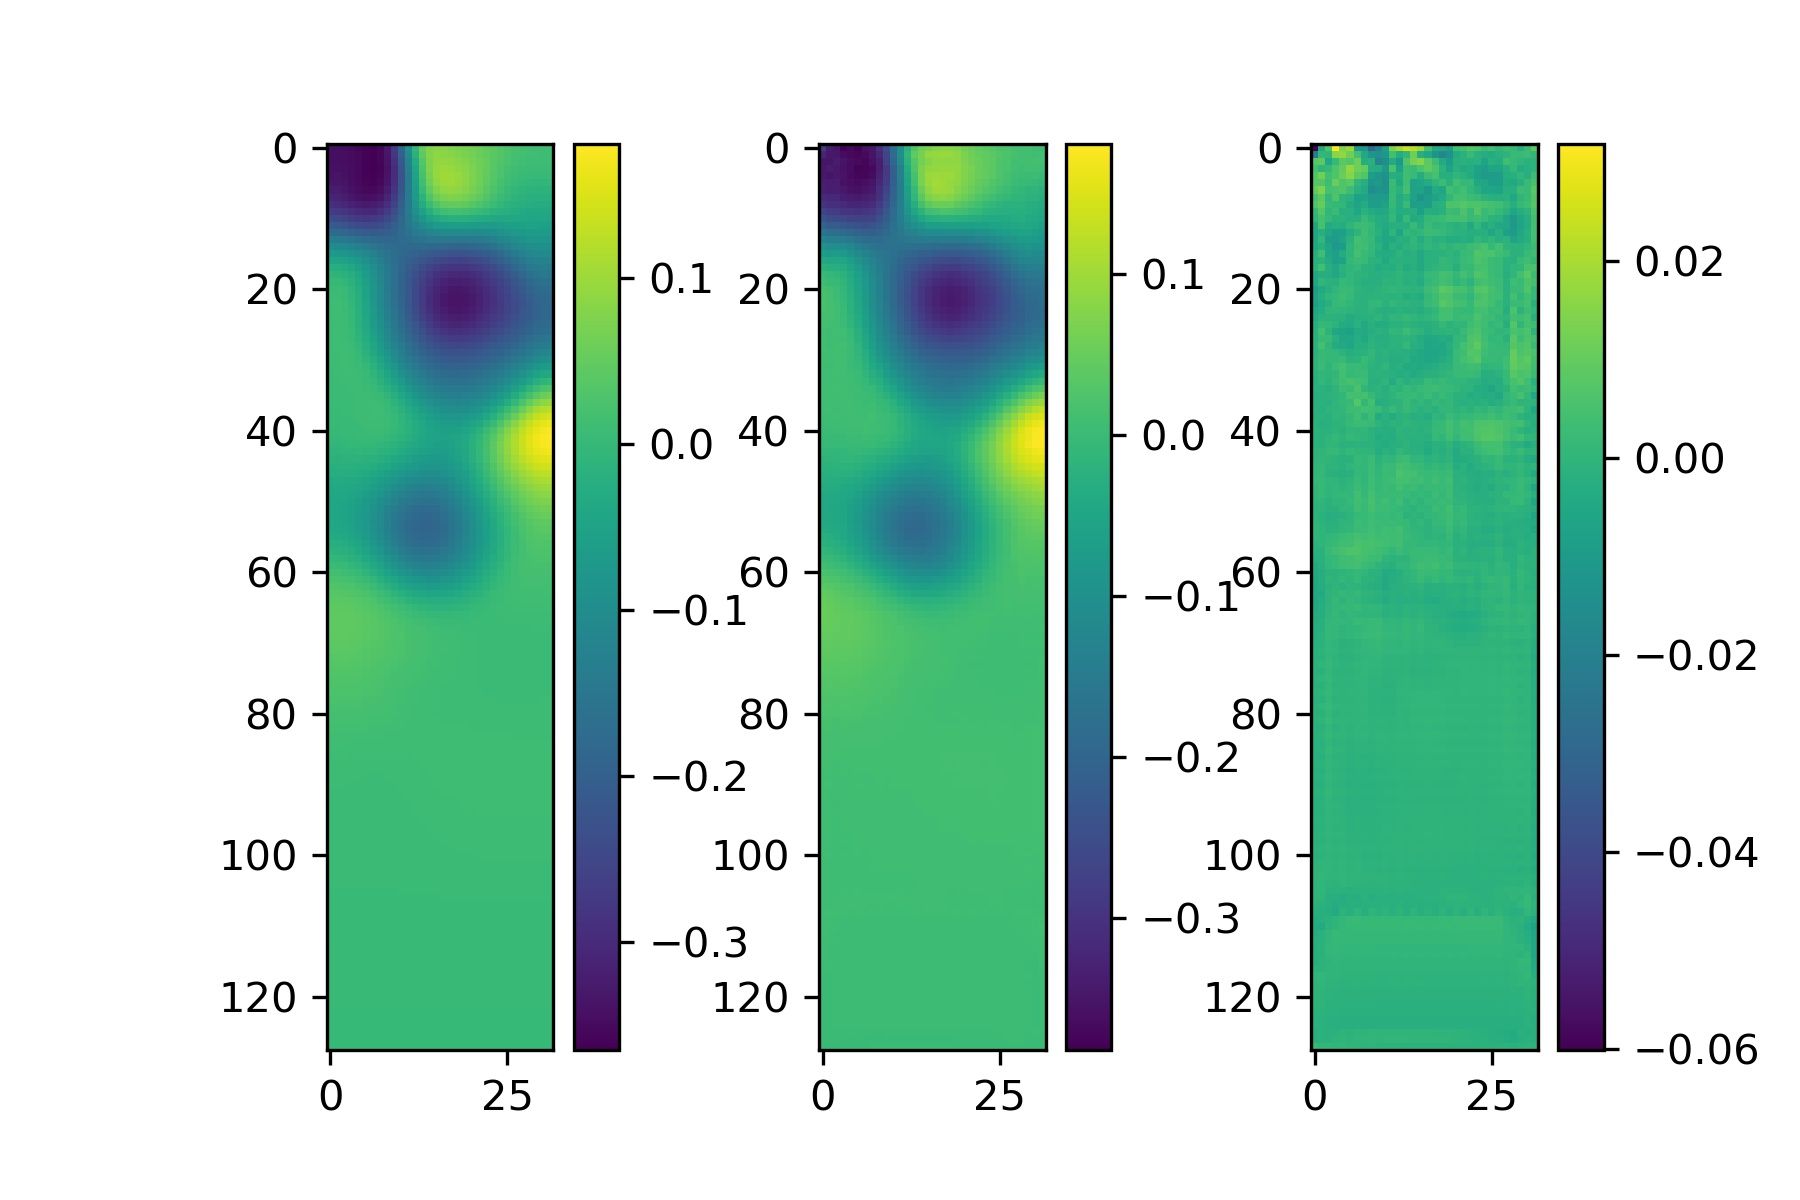
\includegraphics[width=0.9\linewidth]{fig/ns_p.jpg}}
          \caption{Prediction of pressure at time $t=7$; Left: ground truth;
					Middle: prediction; Right: error}
\end{figure}
\end{frame}


\begin{frame}{Future work: Algorithm}
In the algorithmic perspective
	\begin{itemize}
		\item 1. Complete the work on encoder-decoder regularized method to mitigate the
		 distribution mismatch in scientific computing.
		\item 2. Scientific computing + Manifold learning/self-supervised learning.
	\end{itemize}

\end{frame}


\begin{frame}{Future work: Application}
	In terms of application, we will further investigate the following thing:
	\begin{itemize}
		\item 1. Try to implant the best performed algorithm to the problems in fluid
		 mechanics such as turbulence transition and flow separation.
		\item 2. Consider interesting problems in physics such as black holes dynamics,
		 space-time classification in general relativity.
	\end{itemize}

\end{frame}






\end{document}

\begin{frame}{Equivariance in Charge Density Prediction}
    \begin{itemize}
        \item Charge density must be invariant to:
        \begin{align*}
            \rho(\mathbf{r}) &= \rho(R\mathbf{r} + \mathbf{t}) \\
            \text{where } R &\in SO(3), \mathbf{t} \in \mathbb{R}^3
        \end{align*}
        \item For molecular systems, we require:
        \begin{align*}
            \rho(\mathbf{r}) &= \sum_{i} \sum_{l=0}^{\infty} \sum_{m=-l}^{l} c_{ilm} R_{l}(r_i)Y_{lm}(\hat{\mathbf{r}}_i) \\
            \text{where } \hat{\mathbf{r}}_i &= \frac{\mathbf{r} - \mathbf{r}_i}{|\mathbf{r} - \mathbf{r}_i|}
        \end{align*}
        \item Key considerations:
        \begin{itemize}
            \item Rotational equivariance of spherical harmonics
            \item Translation invariance of relative positions
            \item Permutation invariance of identical atoms
        \end{itemize}
    \end{itemize}
\end{frame}

\begin{frame}{Charge3Net: Higher-Order Angular Momentum}
    \begin{columns}
        \column{0.6\textwidth}
        \begin{itemize}
            \item Novel approach using higher-order angular momentum
            \item Key components:
            \begin{itemize}
                \item Spherical harmonics expansion
                \item Radial basis functions
                \item Message passing network
            \end{itemize}
            \item Mathematical formulation:
            \begin{align*}
                \psi_{nlm}(r,\theta,\phi) &= R_{nl}(r)Y_{lm}(\theta,\phi) \\
                \text{where } Y_{lm} &= \sqrt{\frac{2l+1}{4\pi}\frac{(l-m)!}{(l+m)!}}P_l^m(\cos\theta)e^{im\phi}
            \end{align*}
            \item Training objective:
            \begin{align*}
                \mathcal{L}_{\text{ChargE3Net}} &= \frac{1}{n}\sum_{i=1}^n |\rho(\mathbf{r}_i) - \hat{\rho}(\mathbf{r}_i)| \\
                \text{where } n &\text{ is number of grid points}
            \end{align*}
        \end{itemize}
        \column{0.4\textwidth}
        Spherical harmonics visualization
    \end{columns}
\end{frame}

\section{ChargE3Net}


\begin{frame}{ChargE3Net Architecture Overview}
    \begin{itemize}
        \item Based on the E3NN backbone.
        \item Construct two k-d trees to partition the atoms and probes.
        \item Two types of convolutions:
        \begin{itemize}
            \item Conv$_{\text{atom}}$: Bidirectional between atoms
            \begin{equation*}
                \text{Conv}_{\text{atom}}^n(\mathbf{r}_i, X_i^n) = 
                W_1^n (\sum_{j \in \partial(i)}W_2^nX_j^n \otimes R(r_{ij})Y(\mathbf{r}_{ij}))
                + W_3^n X_i^{n}.
            \end{equation*}
            \item Conv$_{\text{probe}}$: From atoms to probes, only contains neighboring
            atoms, no probe-probe interactions.
        \end{itemize}
        \item Training objective:
        \begin{align*}
            \mathcal{L} &= \frac{\sum_{\mathbf{r} \in G} |\rho(\mathbf{r}) - \hat{\rho}(\mathbf{r})|}{
                \sum_{\mathbf{r} \in G} |\rho(\mathbf{r})|}
        \end{align*}
    \end{itemize}
\end{frame}


\begin{frame}{Model performance}
    \begin{itemize}
        \item Vertices:
        \begin{itemize}
            \item Atoms: One-hot encoding of atomic number; reps = Nx0o.
            \item Probe points: Initialized as zero scalar; reps = 1x0o.
        \end{itemize}
        \item Edges:
        \begin{itemize}
            \item Atom-atom: Unidirectional, cutoff 4Å
            \item Atom-probe: Directed from atoms to probes
        \end{itemize}
        \item Periodic boundary conditions supported
    \end{itemize}
    \begin{figure}
        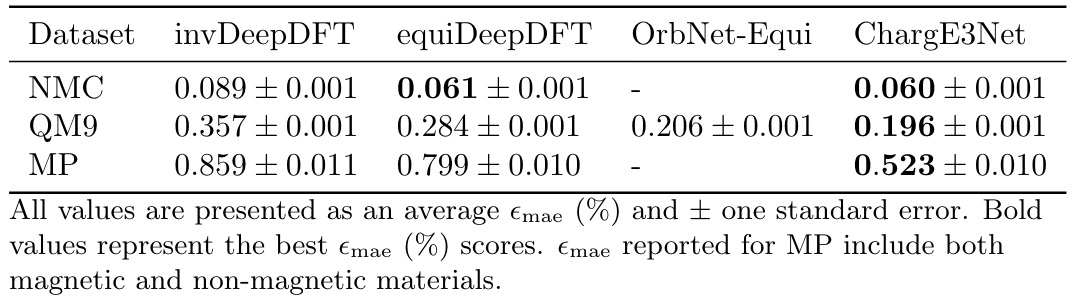
\includegraphics[width=\textwidth]{figures/charge3net_1.jpg}
    \end{figure}
\end{frame}


\begin{frame}{Performance}
    \begin{itemize}
        \item Accelerate DFT calculations: MP materials: 26.7\% reduction;
        GNoME materials: 28.6\% reduction.
        \item Non-self-consistent property prediction:
        \begin{itemize}
            \item 40\% of materials: energy errors < 1 meV/atom
            \item 70\% of materials: forces < 0.03 eV/Å
            \item 76\% of materials: band gaps within chemical accuracy
        \end{itemize}
        \item Linear scaling O(N) with system size.
    \end{itemize}
    \begin{figure}
            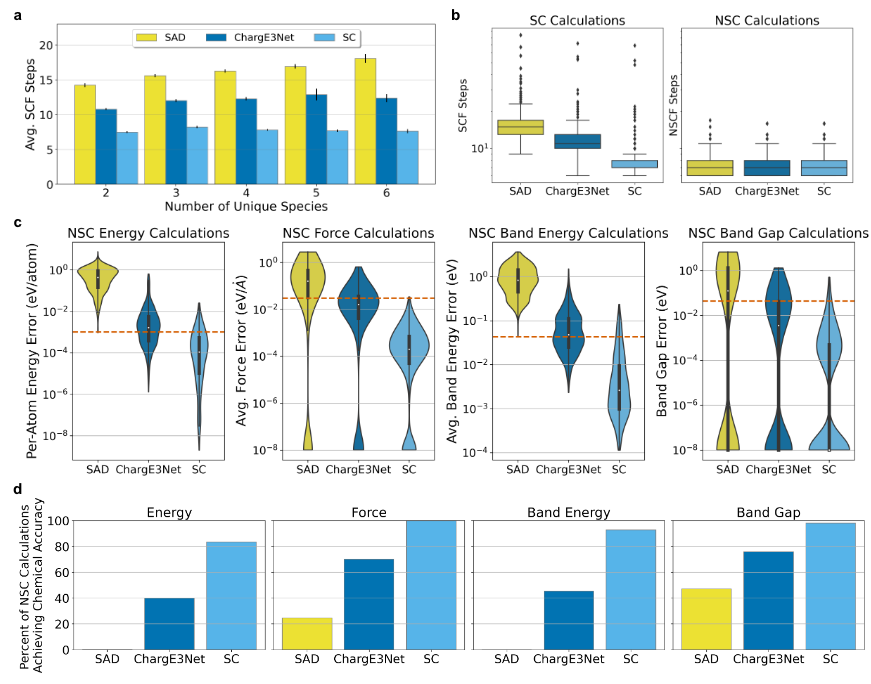
\includegraphics[width=.42\textwidth]{figures/charge3net_2.jpg}
            \caption{}
    \end{figure}
\end{frame}


\begin{frame}{Effect of higher-order features}
    \begin{itemize}
        \item The total dimension of features is N.
        \item With highest order $L$, The dimension of each order is $N/(L + 1)$.
        \item The channel of order $l$ is $N / (L + 1) / (2l + 1)$.
    \end{itemize}
    \begin{figure}
            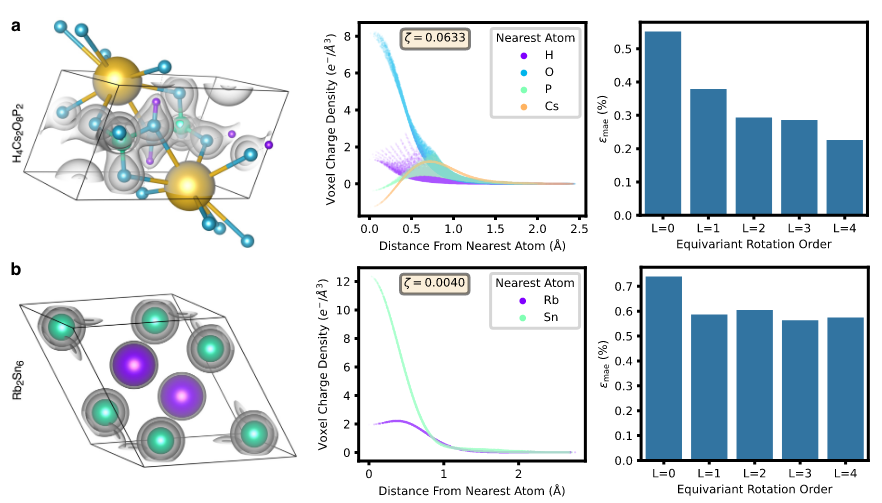
\includegraphics[width=.8\textwidth]{figures/charge3net_3.jpg}
            \caption{}
    \end{figure}
\end{frame}


\begin{frame}{Angular Variance Analysis}
    \begin{itemize}
        \item Performance improvement:
        \begin{itemize}
            \item 44.6\% median improvement for materials with non-metals/metalloids
            \item 23.0\% median improvement for materials with only metals
        \end{itemize}
        \item Metric $\zeta$ for angular variance:
        \[
        \zeta(G) = 1 - \frac{\sum_{\vec{g}_k \in G} |\nabla\rho(\vec{g}_k) \cdot \hat{r}_{ki}|}{\sum_{\vec{g}_k \in G} ||\nabla\rho(\vec{g}_k)||}
        \]
        \item High angular variance materials, e.g. Cs(H2PO4)
        \begin{itemize}
            \item Strong covalent bonding
            \item Significant L=4 improvement
        \end{itemize}
        \item Low angular variance materials, e.g. Rb2Sn6:
        \begin{itemize}
            \item Primarily ionic interactions
            \item Similar L=0 and L=4 performance
        \end{itemize}
    \end{itemize}
\end{frame} 
\section{SCDP: Spherical Channel Density Prediction}

\begin{frame}{SCDP Architecture Overview}
    \begin{itemize}
        \item Basis-based approach with following ingredients:
        \begin{itemize}
            \item Virtual nodes for non-local electronic structures
            \item Even-tempered Gaussian basis sets
            \item High-capacity equivariant spherical channel network (eSCN).
        \end{itemize}
        \item Charge density representation with trainable scale parameters:
        \begin{align*}
            \rho(\mathbf{r}) &= \sum_a \sum_l^{N_a} \sum_{m = -l}^{l} c_{alm}
            \Phi_{\alpha,l,m,\mathbf{r}_a}(\mathbf{r}, s_{al}) \\
            \Phi_{\alpha,l,m,\mathbf{r}_i}(\mathbf{r}, s) &= 
            z_{\alpha,l,s} \exp(-s \cdot \alpha |\mathbf{r} - \mathbf{r}_a|^2) 
            |\mathbf{r} - \mathbf{r}_a|^l Y_{lm}(
                \widehat{\mathbf{r} - \mathbf{r}_a})
        \end{align*}
        \item Model prediction, scaling factors $s_{al} \in (0.5, 2.0)$:
        \begin{align*}
            \{c_{alm}, s_{al}\} &= F(\{(\mathbf{r}_a, Z_a)\}).
        \end{align*}
    \end{itemize}
\end{frame}


\begin{frame}{Virtual Nodes and Basis Sets}
    \begin{itemize}
        \item Virtual nodes:
        \begin{itemize}
            \item Placed at bond midpoints.
            \item Use oxygen basis functions
            \item SE(3)-equivariant placement
        \end{itemize}
        \item Even-tempered Gaussian basis for better accuracy:
        \begin{align*}
            \alpha_k &= \alpha \cdot \beta^k \text{ for } k = 0,1,2,...,N_l
        \end{align*}
        \item  Reducing SO(3) convolution to SO(2): $O(L^6) \rightarrow O(L^3)$.
        \item  The basis set is not orthonormal, the coefficients depend on the
        cutoff radius.
        \item Two-stage training for stability caused by the scale factors
        on the exponent:
        \begin{itemize}
            \item pre-train the model with fixed basis set exponents
            \item fine-tune the prediction model with a small learning rate with
            the learning for scaling factors enabled.
        \end{itemize}
    \end{itemize}
\end{frame}


\begin{frame}{Model Architecture}
    \begin{itemize}
        \item Backbone: eSCN (equivariant spherical channel network)
        \begin{itemize}
            \item $\{x_a\} = \text{eSCN}(\{(\mathbf{r}_a, Z_a)\})$
            \item Complexity: $O(L^3)$ vs $O(L^6)$ for tensor products
            \item Features: Multi-channel spherical harmonics
            \item Example: $128\times0e + 128\times1o + 128\times2e + 128\times3o$
        \end{itemize}
        \item Prediction layers:
        \begin{align*}
            \{c_{alm}, h_i\} &= \text{FullyConnectedTensorProduct}(x_i, x_l) \\
            s_{al} &= \frac{C_1}{1 + \exp(-\text{Linear}(h_i) + \ln C_2)} + C_3
            \in [C_1, C_3].
        \end{align*}
        \item Training objective:
        \begin{align*}
            \mathcal{L} &= \mathbb{E}_{\mathbf{r}\in\text{Data}}[|\rho(\mathbf{r}) - \hat{\rho}(\mathbf{r})|]
        \end{align*}
    \end{itemize}
\end{frame}


% \begin{frame}{pseudocode}
%     \begin{figure}
%         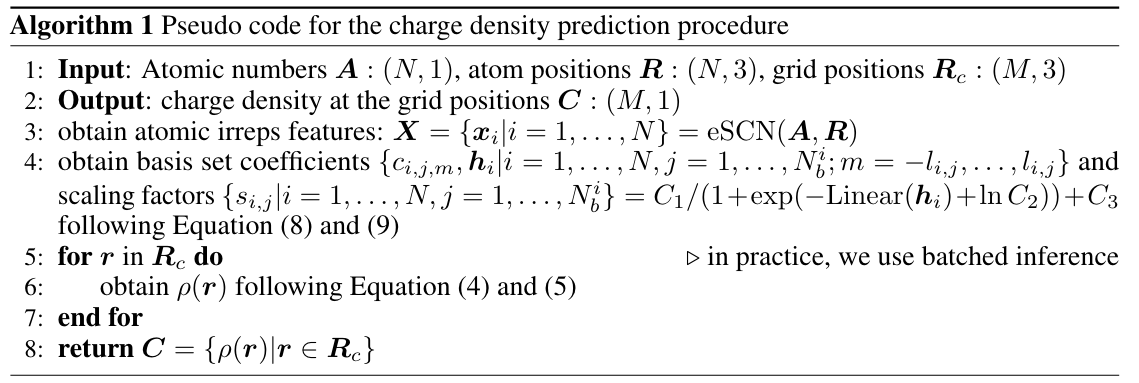
\includegraphics[width=\textwidth]{figures/scdp_3.jpg}
%     \end{figure}
% \end{frame}


\begin{frame}{Performance Analysis}
    \begin{itemize}
        \item NMAE: 0.178\% on QM9 test set
        \item 31.7x faster than ChargE3Net
        \item Flexible accuracy-efficiency trade-off
    \end{itemize}
    \begin{figure}
        \begin{subfigure}{0.48\textwidth}
        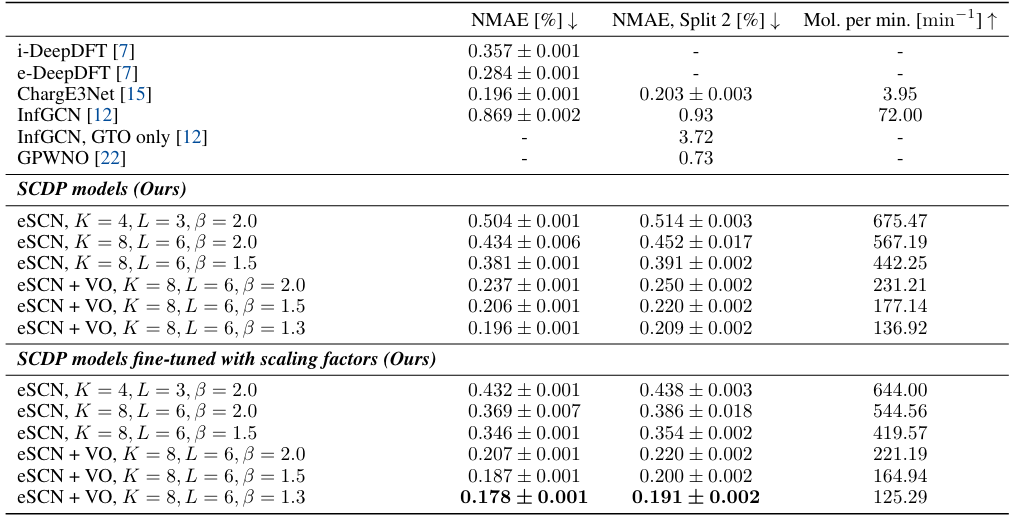
\includegraphics[width=\textwidth]{figures/scdp_2.jpg}
    \end{subfigure}
    \begin{subfigure}{0.48\textwidth}
        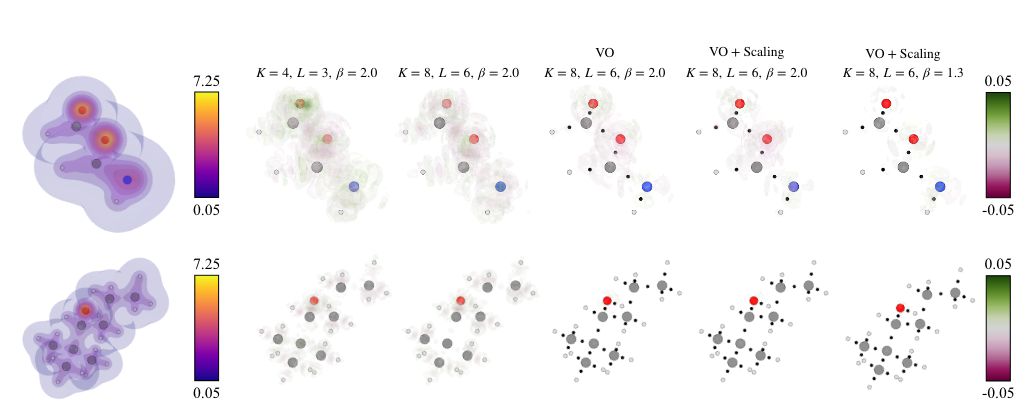
\includegraphics[width=\textwidth]{figures/scdp_1.jpg}
    \end{subfigure}
    \end{figure}
\end{frame}


\begin{frame}{Uni3D-AR: Foundation Model Adaptation}
    \begin{itemize}
        \item Grid-based tokenization
        \begin{itemize}
            \item 3D voxel grid representation
            \item Multi-scale feature extraction
            \item Hierarchical attention
        \end{itemize}
        \item Key innovations:
        \begin{itemize}
            \item Adaptive grid resolution
            \item Local-global feature fusion
            \item Position-aware attention
        \end{itemize}
        \item Based on transformer architecture
        \item Key features:
        \begin{itemize}
            \item Pre-training on large datasets
            \item Fine-tuning for charge density
            \item Multi-task learning capability
        \end{itemize}
        \item Training objective:
        \begin{align*}
            \mathcal{L}_{\text{Uni3D-AR}} &= \mathcal{L}_{\text{main}} + \lambda\mathcal{L}_{\text{aux}} \\
            \text{where } \mathcal{L}_{\text{main}} &= \text{Masked next-token prediction} \\
            \mathcal{L}_{\text{aux}} &= \text{Property prediction loss}
        \end{align*}
    \end{itemize}
\end{frame}
\section{Uni-3DAR: Unified 3D Generation and Understanding}

\begin{frame}{Uni-3DAR Overview}
    \begin{itemize}
        \item Tokenization-based approach
        \item Key components:
        \begin{itemize}
            \item Hierarchical octree compression
            \item Fine-grained structural tokenization
            \item Masked next-token prediction
        \end{itemize}
        \item Unifies:
        \begin{itemize}
            \item 3D structure generation
            \item Property prediction
            \item Multi-modal tasks
        \end{itemize}
    \end{itemize}
\end{frame}

\begin{frame}{Hierarchical Tokenization}
    \begin{itemize}
        \item Octree-based compression:
        \begin{itemize}
            \item Coarse-to-fine subdivision
            \item Non-empty cell detection
            \item Level-wise tokenization
        \end{itemize}
        \item Fine-grained tokenization:
        \begin{itemize}
            \item Atom types and positions
            \item In-cell coordinate discretization
            \item Structural details
        \end{itemize}
        \item 2-level subtree compression:
        \begin{itemize}
            \item 8 subcells → 1 token
            \item 256 possible states
            \item 8x reduction in tokens
        \end{itemize}
    \end{itemize}
\end{frame}

\begin{frame}{Masked Next-Token Prediction}
    \begin{itemize}
        \item Challenge: Dynamic token positions
        \item Solution:
        \begin{itemize}
            \item Token duplication
            \item Masked token replacement
            \item Position-aware prediction
        \end{itemize}
        \item Benefits:
        \begin{itemize}
            \item Handles varying token positions
            \item Maintains causal sampling
            \item Improves prediction accuracy
        \end{itemize}
    \end{itemize}
\end{frame}

\begin{frame}{Unified Framework}
    \begin{itemize}
        \item Single-frame generation:
        \begin{itemize}
            \item Unconditional generation
            \item Property-conditioned generation
            \item Text-guided generation
        \end{itemize}
        \item Multi-frame generation:
        \begin{itemize}
            \item Molecular dynamics
            \item Pocket-based generation
            \item Frame-by-frame prediction
        \end{itemize}
        \item Understanding tasks:
        \begin{itemize}
            \item Token-level properties
            \item Structure-level properties
            \item Cross-modal tasks
        \end{itemize}
    \end{itemize}
\end{frame}

\begin{frame}{Performance Analysis}
    \begin{itemize}
        \item Generation tasks:
        \begin{itemize}
            \item Up to 256\% relative improvement
            \item 21.8x faster inference
            \item Better quality and diversity
        \end{itemize}
        \item Understanding tasks:
        \begin{itemize}
            \item Competitive with specialized models
            \item Effective transfer learning
            \item Multi-task learning benefits
        \end{itemize}
    \end{itemize}
\end{frame}

\begin{frame}{Efficiency Optimizations}
    \begin{itemize}
        \item Training:
        \begin{itemize}
            \item FlashAttention with bfloat16
            \item Sequence packing
            \item Efficient memory usage
        \end{itemize}
        \item Inference:
        \begin{itemize}
            \item KV-cache acceleration
            \item Paired token generation
            \item GPU utilization optimization
        \end{itemize}
    \end{itemize}
\end{frame}

\begin{frame}{Cross-Modal Applications}
    \begin{itemize}
        \item Protein folding:
        \begin{itemize}
            \item Sequence to structure
            \item Multi-frame generation
            \item Property prediction
        \end{itemize}
        \item Crystal structure prediction:
        \begin{itemize}
            \item PXRD-guided generation
            \item NMR signal conditioning
            \item Property optimization
        \end{itemize}
    \end{itemize}
\end{frame} 

\begin{frame}{Performance Comparison}
    \begin{table}[h]
        \centering
        \begin{tabular}{lccc}
            \toprule
            Model & MAE & RMSE & Training Time \\
            \midrule
            Charge3Net & 0.012 & 0.015 & 24h \\
            SCDP & 0.008 & 0.010 & 48h \\
            Uni3D-AR & 0.006 & 0.008 & 72h \\
            \bottomrule
        \end{tabular}
        \caption{Performance metrics across models}
    \end{table}
\end{frame}

\begin{frame}{Future Directions}
    \begin{columns}
        \column{0.5\textwidth}
        \begin{itemize}
            \item Integration with foundation models
            \begin{itemize}
                \item Pre-training strategies
                \item Transfer learning
                \item Multi-task learning
            \end{itemize}
            \item Technical challenges:
            \begin{itemize}
                \item Computational efficiency
                \item Data requirements
                \item Model interpretability
            \end{itemize}
        \end{itemize}
        \column{0.5\textwidth}
        Potential research directions
    \end{columns}
\end{frame}

\end{document} 